%!TEX program = xelatex
% 【關鍵設定】fontset=none 代表不使用預設字型，依模板設定字型
\documentclass[fontset=none, a4paper, 12pt]{ctexart} 

% ==========================================
% 1. 套件載入區
% ==========================================
\usepackage{geometry}
\usepackage{longtable}
\usepackage{fontspec}
\usepackage{setspace}
\usepackage{titlesec}
\usepackage{titletoc}
\usepackage{tocloft}
\usepackage{fancyhdr}
\usepackage{graphicx}
\usepackage{caption}
% 圖表與標題間距壓縮
\captionsetup[figure]{skip=4pt}
\captionsetup[table]{skip=4pt}
\setlength{\intextsep}{7pt}
\setlength{\textfloatsep}{7pt}
\setlength{\floatsep}{7pt}
\usepackage[hidelinks]{hyperref}
\usepackage{booktabs}
\usepackage{float}
\usepackage{amsmath}
\usepackage{amssymb}
\usepackage{tabularx}
\usepackage{placeins}
\usepackage{needspace}
\usepackage{algorithm}
\usepackage{algpseudocode}
\floatname{algorithm}{演算法}
\usepackage{makecell}
\usepackage{array}
\usepackage{pdflscape}
\usepackage{rotating}
\usepackage{pdfpages}
\sloppy

% ===== refs.bib 管理文獻設定 =====
\usepackage[
  backend=biber,
  style=numeric,
  sorting=none,
  maxbibnames=99,
  giveninits=true,
  doi=true,
  url=true,
  isbn=false
]{biblatex}

\addbibresource{refs.bib}
\DeclareNameAlias{default}{family-given}
\DeclareDelimFormat{finalnamedelim}{\addcomma\space\&\space}
\renewbibmacro{in:}{%
  \ifentrytype{article}{}{\printtext{\bibstring{in}\intitlepunct}}}
\DeclareFieldFormat[article]{title}{#1}
\DeclareFieldFormat[inproceedings]{title}{#1}
\DeclareFieldFormat[misc]{title}{#1}

% ==========================================
% 2. 字型設定
% ==========================================
\setCJKmainfont{kaiu.ttf}[
    AutoFakeBold=2.5,
    AutoFakeSlant=0.3
]
\setmainfont{TeX Gyre Termes}
\newCJKfontfamily\coverzh{kaiu.ttf}[
    AutoFakeBold=2.5,
    AutoFakeSlant=0.3
]
\newfontfamily\coveren{Times New Roman}

% ==========================================
% 3. 版面與格式設定
% ==========================================
\geometry{a4paper, top=3cm, bottom=3cm, left=3cm, right=3cm}
\pagestyle{plain} 

% 圖表標題中文化
\captionsetup[figure]{name=圖}
\captionsetup[table]{name=表}
\ctexset{bibname = {參考文獻}}

% 章節標題格式
\titleformat{\section}[block]{\centering\fontsize{20}{24}\selectfont\bfseries}{\thesection}{1em}{}
\titleformat{\subsection}[block]{\fontsize{16}{20}\selectfont\bfseries}{\thesubsection.}{1em}{}
\titleformat{\subsubsection}[block]{\fontsize{14}{18}\selectfont\bfseries}{\thesubsubsection.}{1em}{}

% 編號格式
\renewcommand{\thesection}{第\chinese{section}章}
\renewcommand{\thesubsection}{\arabic{section}.\arabic{subsection}}
\renewcommand{\thesubsubsection}{\arabic{section}.\arabic{subsection}.\arabic{subsubsection}}

% 目錄設定
\renewcommand{\contentsname}{目錄}
\renewcommand{\listtablename}{表目錄}
\renewcommand{\listfigurename}{圖目錄}

\renewcommand{\cfttoctitlefont}{\hfill\Large\bfseries}
\renewcommand{\cftaftertoctitle}{\hfill\null}
\renewcommand{\cftlottitlefont}{\hfill\Large\bfseries}
\renewcommand{\cftafterlottitle}{\hfill\null}
\renewcommand{\cftloftitlefont}{\hfill\Large\bfseries}
\renewcommand{\cftafterloftitle}{\hfill\null}

\setlength{\cftbeforetoctitleskip}{0pt}
\setlength{\cftaftertoctitleskip}{1.2em}
\setlength{\cftbeforelottitleskip}{0pt}
\setlength{\cftafterlottitleskip}{1.2em}
\setlength{\cftbeforeloftitleskip}{0pt}
\setlength{\cftafterloftitleskip}{1.2em}

\renewcommand{\cftsecleader}{\cftdotfill{\cftdotsep}}
\renewcommand{\cftsubsecleader}{\cftdotfill{\cftdotsep}}
\renewcommand{\cftsubsubsecleader}{\cftdotfill{\cftdotsep}}

\renewcommand{\cftsecfont}{\bfseries}
\renewcommand{\cftsecpagefont}{\bfseries}
\setlength{\cftbeforesecskip}{1.5em}

\begin{document}

% ==========================================
% 封面（不顯示頁碼）
% ==========================================
\newgeometry{
    a4paper,
    top=3cm,
    bottom=3cm,
    left=3cm,
    right=3cm
}

\begin{titlepage}
    \centering
    \thispagestyle{empty}
    \vspace*{0.7cm}

    {\coverzh
    \fontsize{20pt}{28pt}\selectfont
    \begingroup
    \xeCJKsetup{CJKglue=\hskip -1.55pt}
    \makebox[\textwidth][c]{%
        國立中興大學人工智慧與資料科學碩士在職學位學程%
    }
    \endgroup
    \par}

    \vspace{0.35cm}

    {\coverzh
    \fontsize{20pt}{28pt}\selectfont
    碩士學位論文\par}

    \vspace{2.5cm}

    {\coverzh
    \fontsize{20pt}{29pt}\selectfont
    半導體製程冷卻水系統之異常行為辨識\\與智慧預先檢測研究\par}

    \vspace{0.75cm}

    {\coveren
    \fontsize{18pt}{24pt}\selectfont
    \makebox[\textwidth][c]{%
        Research on Abnormal Behavior Detection and Intelligent Predetection%
    }\par
    \makebox[\textwidth][c]{%
        of Process Cooling Water Systems in Semiconductor Manufacturing%
    }\par}

    \vspace{2.4cm}

    {\coverzh
    \fontsize{20pt}{28pt}\selectfont
    指導教授：
    \hspace{0.3em}
    林長鋆
    \hspace{0.1em}
    {\coveren Chang-Yun Lin}\par}

    \vspace{0.35cm}

    {\coverzh
    \fontsize{20pt}{28pt}\selectfont
    研究生：
    \hspace{0.3em}
    陳宥興
    \hspace{0.1em}
    {\coveren You-Xing Chen}\par}

    \vspace{2.0cm}

    {\coverzh
    \fontsize{20pt}{28pt}\selectfont
    中華民國一百一十五年十一月\par}

\end{titlepage}

\restoregeometry
\clearpage

% ==========================================
% 口試審核頁（不編頁碼）
% ==========================================
\thispagestyle{empty}
\vspace*{\fill}
\begin{center}
    \Large 口試審核頁預留
\end{center}
\vspace*{\fill}
\clearpage

% ==========================================
% 誌謝
% ==========================================
\clearpage
\pagenumbering{gobble}
\pagestyle{empty}

\begin{center}
    \large\bfseries 誌謝
\end{center}
\vspace{0.5em}

碩士研究歷程的完成，首先由衷感謝指導教授林長鋆博士在人工智慧、統計品質管制與工業物聯網架構領域的悉心指導與鞭策。老師嚴謹的治學態度、對理論公式閉式解與實體硬體工程落地並重之堅持，奠定了本論文兼具學術深度與工業實用性的基石。

特別感謝產業界與實驗室同儕在工業通訊協定、Modbus TCP 暫存器架構與分散式微秒級推論驗證過程中的寶貴交流。感謝家人的無條件支持與體諒，使我得以在長程全廠 1,600 次自動化壓力測試與模型硬化調校過程中保持專注，終能順利完成學位論文。謹將本研究成果獻給所有支持與關心我的師長、家人與摯友。

\vspace{2em}
\begin{flushright}
陳宥興　謹誌\\
中華民國一百一十五年十一月
\end{flushright}

% ==========================================
% 前半部：羅馬數字編碼 (i, ii, iii...)
% ==========================================
\clearpage
\pagestyle{plain}
\pagenumbering{roman}
\setcounter{page}{1}

% ==========================================
% 中文摘要
% ==========================================
\phantomsection
\addcontentsline{toc}{section}{摘要}
\begin{center}
\large\bfseries 摘要
\end{center}
\vspace{0.5em}

現代先進半導體晶圓廠中，製程冷卻水（Process Cooling Water, PCW）為極紫外光微影（EUV）、乾式電漿蝕刻與化學機械研磨等極端製程設備之散熱命脈。傳統廠務監控仰賴靜態閾值警報，僅能在感測器突破工程上限時事後通報，常因緩慢水力漂移累積導致設備過溫跳機，造成動輒數百萬美元之晶圓報廢損失。

本研究針對雙層晶圓廠空間拓撲（2F Cleanroom 與 1F Sub-Fab），提出一套整合「物理水力學流阻守恆（Darcy-Weisbach / Colebrook-White）」與「二項分佈時序漂移檢定（Binomial Anomaly Density）」之智慧預先檢測演算法。模型在嚴格因果滑動視窗下，推導對稱雙向普通最小二乘法（OLS）斜率與到限時間（Time-To-Limit, TTL）之封閉解析解，並實作七層工業級硬化防護防線。經實體主機探針（Apple M5 10-Core，16GB RAM）實測，演算法平均延遲僅 $89.36\ \mu\mathrm{s}$，單核吞吐量達 11,190 ops/s；在全廠 8 套獨立循環、80 個 Submain 與 160 顆壓力感測器之 1,600 場次長程壓力測試中，模型達成 100.0\% 召回率、98.54\% 精確率與 0.9926 之 F1-Score，並提供平均 18.23 分鐘之故障提前預警量，有效消弭被動閾值之滯後風險。

\vspace{1em}
\noindent \textbf{關鍵詞：}製程冷卻水系統、流體力學模型、二項分佈檢定、普通最小二乘法、到限時間預警、微秒級延遲、半導體廠務

\newpage

% ==========================================
% 英文摘要 (Abstract)
% ==========================================
\phantomsection
\addcontentsline{toc}{section}{Abstract}
\begin{center}
\large\bfseries Abstract
\end{center}
\vspace{0.5em}

In modern semiconductor fabrication facilities (Fabs), the Process Cooling Water (PCW) system represents a mission-critical utility for dissipating massive heat flux generated by extreme process chambers, such as EUV lithography, plasma dry etching, and chemical mechanical planarization (CMP). Traditional SCADA systems rely strictly on reactive threshold alarms, triggering only after pressures exceed boundary limits, which leaves zero buffer time to prevent catastrophic wafer scrap.

This thesis presents a physics-informed intelligent predetection framework tailored for dual-level fab spatial topologies (2F Cleanroom and 1F Sub-Fab). By coupling Darcy-Weisbach and Colebrook-White hydrodynamic flow resistance formulations with a discrete binomial anomaly density test, the system detects micro-drifts under strict causal sliding window constraints. Closed-form expressions for symmetric bilateral Ordinary Least Squares (OLS) regression slopes and Time-To-Limit (TTL) metrics are derived, accompanied by a 7-layer industrial false-alarm suppression pipeline. Hardware-probed benchmarks on an Apple M5 10-core architecture demonstrate a mean pipeline latency of $89.36\ \mu\mathrm{s}$ and a throughput of 11,190 ops/s. Rigorous plant-wide automated stress testing across 8 closed loops, 80 submains, and 160 pressure transmitters (1,600 operational test runs) demonstrates a 100.0\% recall, 98.54\% precision, and an F1-score of 0.9926, providing a mean advance warning lead time of 18.23 minutes before reaching engineering limits.

\vspace{1em}
\noindent \textbf{Keywords:} Process Cooling Water (PCW), Hydrodynamic Modeling, Binomial Anomaly Test, Ordinary Least Squares, Time-To-Limit, Microsecond Latency, Semiconductor Manufacturing

\newpage

% ==========================================
% 目錄 / 表目錄 / 圖目錄
% ==========================================
\phantomsection
\addcontentsline{toc}{section}{目錄}
\tableofcontents
\newpage

\phantomsection
\addcontentsline{toc}{section}{表目錄}
\listoftables
\newpage

\phantomsection
\addcontentsline{toc}{section}{圖目錄}
\listoffigures
\newpage

% ==========================================
% 正文：阿拉伯數字頁碼 1, 2, 3...
% ==========================================
\clearpage
\pagenumbering{arabic}
\setcounter{page}{1}
\begin{doublespace}

% ============================================================
% 第一章 緒論
% ============================================================
\section{緒論}

\subsection{半導體晶圓廠空間拓撲與製程分區}
現代先進半導體晶圓廠（Fab）採用多樓層空間分區結構，將精密生產設備與重型廠務公用系統實體隔離，以維持最高等級無塵潔淨度並抑制機械振動干擾。如圖~\ref{fig:fab_layout} 所示，全廠主要劃分為三大空間層級：
\begin{enumerate}
    \item \textbf{2F Cleanroom（無塵室生產層）}：配置 PCW01～PCW04 迴路，專屬供應微影（Lithography, EUV/ArFi）、乾式電漿蝕刻（Dry Etching）及高溫擴散氧化（Diffusion）等關鍵核心製程。此區機台對流體壓力脈動與水阻變化極為敏感。
    \item \textbf{1F Sub-Fab（廠務輔助層）}：配置 PCW05～PCW08 迴路，負責化學氣相沉積（CVD）、物理氣相沉積（PVD）、化學機械研磨（CMP）及濕式化學清洗（Wet Cleaning）等重負載設備。
    \item \textbf{CUB（中央廠務大樓, Central Utility Building）}：安置集中式主冷水機組（Chillers）、板式熱交換器（PHE）、離心式變頻主泵群（VFD Primary Pumps）及差壓旁通調度閥，構成全廠冷卻能源中樞。
\end{enumerate}

\begin{figure}[H]
    \centering
    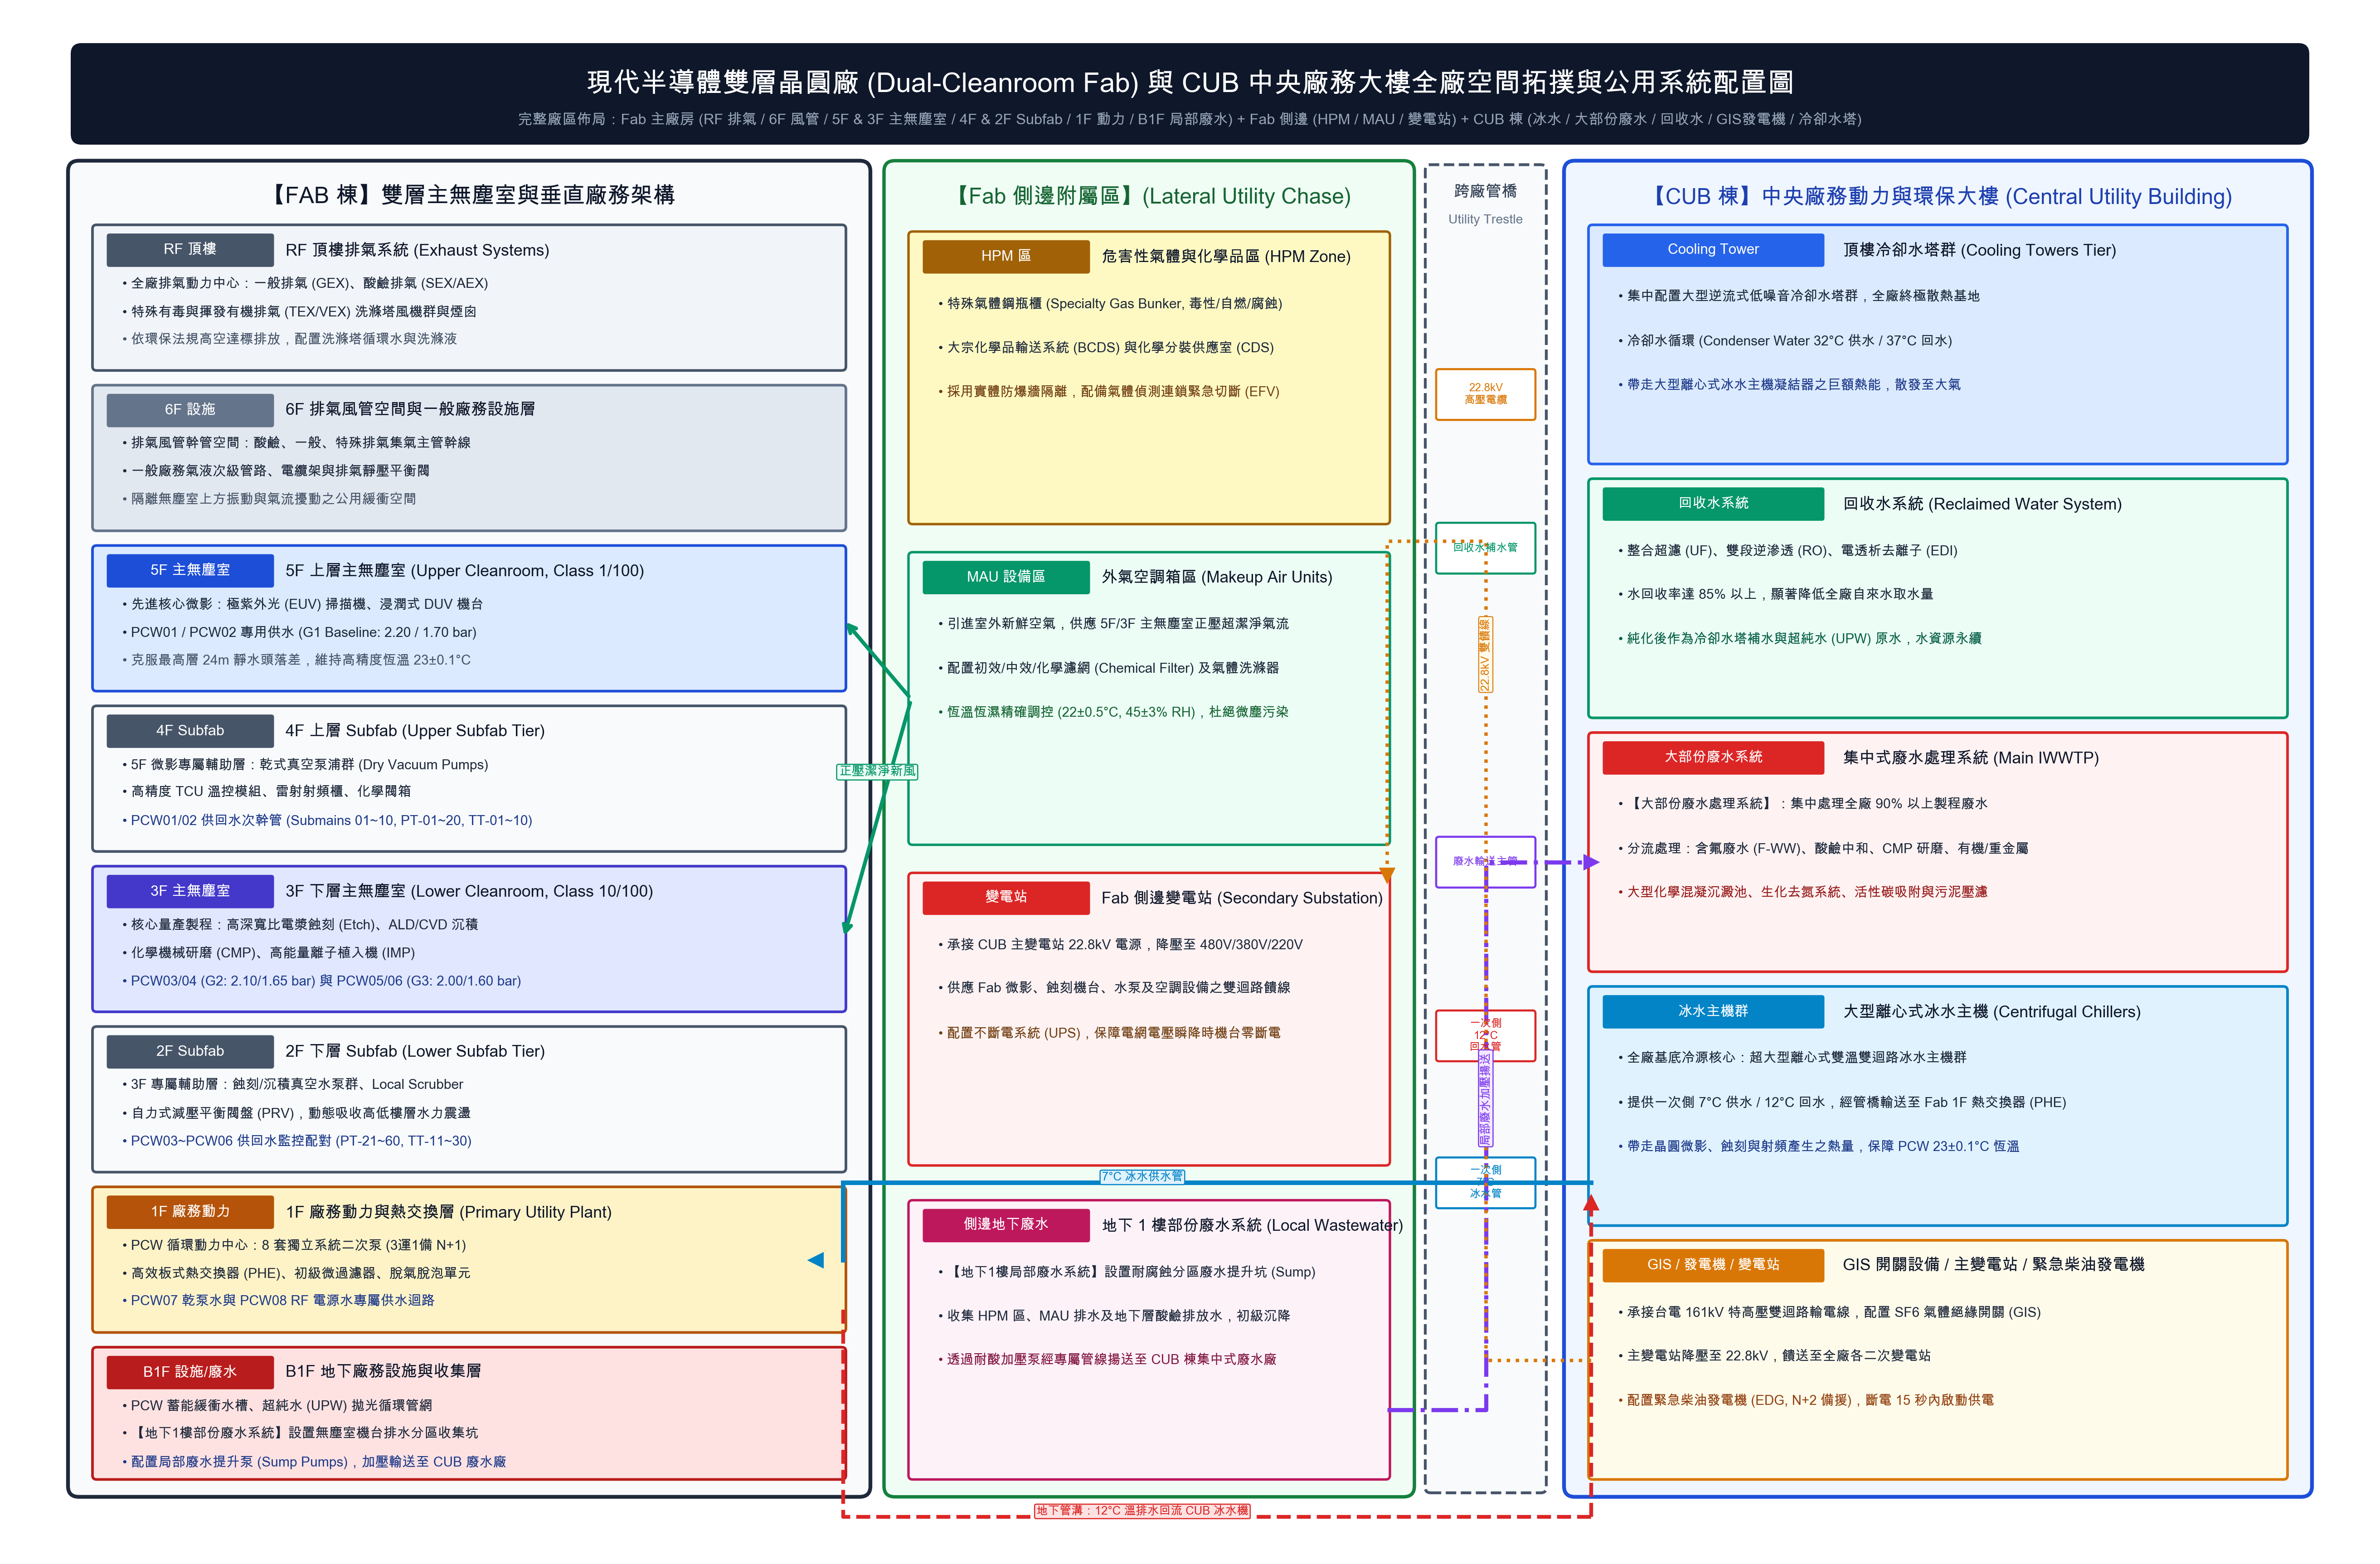
\includegraphics[width=0.88\textwidth,keepaspectratio]{picture/fig_fab_vertical_layout.png}
    \caption{半導體雙層晶圓廠（Cleanroom / Sub-Fab / CUB）空間拓撲與 PCW 立管佈局圖}
    \label{fig:fab_layout}
\end{figure}

\subsection{生產階段冷卻負載特性與嚴苛容許度}
半導體各生產階段之熱流密度與製程保護規範具有顯著差異，冷卻水系統必須滿足極度嚴苛的穩定性要求：
\begin{itemize}
    \item \textbf{極紫外光微影（EUV）}：真空鏡室與大功率射頻源持續產生高達數十千瓦之集中熱負載，冷卻水壓波動必須控制在 $\pm 0.05\ \mathrm{bar}$ 以內，以避免微振影響奈米級疊對精準度（Overlay Accuracy）。
    \item \textbf{乾式電漿蝕刻}：電漿放電反應腔體需維持精確恆溫，回水背壓異常將導致晶圓邊緣熱梯度失衡，直接破壞蝕刻均勻度。
    \item \textbf{薄膜沉積（CVD/PVD）}：高頻 RF 匹配電路與靶材冷卻需連續大流量供水，濾網阻塞或微小洩漏將引發高溫連鎖保護跳機。
    \item \textbf{化學機械研磨（CMP）}：研磨盤動態摩擦生熱具突發週期性，需具備動態補償與高壓緩衝能力。
\end{itemize}

\subsection{PCW 系統架構配置、功能目的與運作程序}
本研究針對現代 12 吋先進製程晶圓廠標準規模進行建模與實體驗證：
\begin{enumerate}
    \item \textbf{架構配置}：全廠共建置 8 套獨立封閉循環迴路（PCW01 至 PCW08）。每套迴路各配置 10 個次幹管分支（Submain 01 至 Submain 10），全廠共計 80 個 Submain。每個 Submain 皆安裝供水（Supply）與回水（Return）雙壓力計，全廠實體監控測點涵蓋 160 支壓力計（PT-01～PT-160）、80 支溫度計（TT）與 16 支主流量計（FT）。
    \item \textbf{參數分組與工程門檻}：如表~\ref{tab:pcw_groups} 所示，全廠依機台負載特性劃分為四大參數分組（G1～G4），各自定義嚴格的常態運轉基準線（Baseline）與四級警報安全門檻（HiHi, Hi, Lo, LoLo）。
    \item \textbf{功能目的}：提供高純度去離子冷卻水，維持供水溫度在 $22.0 \pm 0.5^\circ\mathrm{C}$，並維持穩定供回水壓差，即時吸收製程高熱。
    \item \textbf{運作程序}：CUB 離心冷卻泵增壓 $\to$ 垂直立管（Riser）向上輸送至 1F/2F 各區 $\to$ Submain 調節閥二次配水至機台熱交換盤管 $\to$ 吸熱後匯入回水集水管 $\to$ 進入脫氣器與微米級濾網 $\to$ 流經一次板式換熱器降溫，完成封閉式再循環。
\end{enumerate}

\begin{table}[H]
\centering
\caption{PCW 八套獨立循環系統四大分組基準線與安全限值配置表}
\label{tab:pcw_groups}
\footnotesize
\renewcommand{\arraystretch}{1.15}
\setlength{\tabcolsep}{6pt}
\begin{tabularx}{0.96\textwidth}{cccccccc}
\toprule
\textbf{分組代碼} & \textbf{涵蓋迴路} & \textbf{所屬樓層} & \textbf{Baseline (bar)} & \textbf{HiHi (bar)} & \textbf{Hi (bar)} & \textbf{Lo (bar)} & \textbf{LoLo (bar)} \\
\midrule
Group 1 & PCW01, PCW02 & 2F Cleanroom & 1.50 & 1.80 & 1.70 & 1.30 & 1.20 \\
Group 2 & PCW03, PCW04 & 2F Cleanroom & 1.90 & 2.20 & 2.10 & 1.70 & 1.50 \\
Group 3 & PCW05, PCW06 & 1F Sub-Fab   & 2.50 & 2.80 & 2.70 & 2.30 & 2.20 \\
Group 4 & PCW07, PCW08 & 1F Sub-Fab   & 2.10 & 2.40 & 2.30 & 1.90 & 1.80 \\
\bottomrule
\end{tabularx}
\end{table}

\subsection{現行被動閾值監控痛點與研究目標}
現行工業 SCADA 系統普遍遵循靜態上下限（Threshold Limit）報警邏輯，存在三大根本瓶頸：
\begin{enumerate}
    \item \textbf{被動滯後性}：警報觸發瞬間壓力數值已突破安全邊界，操作人員缺乏防禦緩衝時間（Zero Lead Time），只能採取緊急停機或事後搶修。
    \item \textbf{慢速水力漂移盲區}：濾網漸進阻塞或閥門微幅洩漏表現為每分鐘低於 $0.005\ \mathrm{bar}$ 的緩慢漂移，傳統閾值在數十分鐘內無法辨識，直到累積成重大失壓。
    \item \textbf{高頻擾動誤報干擾}：相鄰機台閥件啟閉引起之瞬態水錘脈衝，極易造成單點瞬時越界誤報，導致「警報疲勞（Alarm Fatigue）」。
\end{enumerate}
針對上述痛點，本研究目標在於建構結合物理水力學守恆與統計機率推論之智慧預測模型，在感測數據突破邊界前 15～30 分鐘提供高可靠度的預警時間（TTL），從根本上變更半導體廠務的運維模式。

% ============================================================
% 第二章 文獻探討與基礎理論
% ============================================================
\clearpage
\section{文獻探討與基礎理論}

\subsection{半導體廠務冷卻水監控與 ISA-18.2 警報管理規範}
國際自動化學會（ISA）於 ANSI/ISA-18.2 標準中明確指出~\cite{isa1822016}，健全的工業警報系統應具備「相關性（Relevant）」、「獨特性（Unique）」與「及時性（Timely）」。Smith 等人~\cite{smith2021facility} 研究先進 EUV 微影廠務設施指出，熱管理系統之非預期停機有超過 60\% 源於次幹管流動阻塞與感測器零點漂移。現有 SCADA 介面雖然具備完善的狀態顯示，但缺乏動態趨勢推論能力，極易違反 ISA-18.2 規範中關於警報洪流抑制之準則。

\subsection{統計製程管制與傳統時序迴歸之侷限}
統計製程管制（SPC）廣泛應用於製造品質監控~\cite{montgomery2020statistical}，其中指數加權移動平均（EWMA）對微小偏移具備一定敏感度。然而，EWMA 在工業封閉循環管網中面臨兩大困難：其一，冷卻水管網受機台啟閉負載影響，背景常態值並非定常分佈；其二，EWMA 僅輸出統計控制量，無法直接輸出物理意義明確之預警提前量（Lead Time）或預估到限時間（Time-To-Limit）。另一方面，單純資料驅動之機器學習模型常受資料外推漂移影響，缺乏流體物理守恆約束，易在非穩態工況下產生虛假警報。

\subsection{物理先驗與資料驅動結合之混合預測模型}
為克服純統計或純物理模型之缺點，Caballero 等人~\cite{caballero2026predictive} 與 Li 等人~\cite{li2024prognostics} 倡導將物理系統先驗知識（Physics-Informed Prior）融入資料驅動推論管線。Lin 等人~\cite{lin2023hydraulic} 針對雙層晶圓廠冷卻水之動態水力學建模證實，結合 Darcy-Weisbach 阻力方程與水力壓降分佈能有效約束資料搜尋空間。本研究依循此一理論脈絡，建構兼具物理可解釋性與微秒級即時推論效能之水力學異常預檢模型。

% ============================================================
% 第三章 水力學模型與異常行為推論演算法
% ============================================================
\clearpage
\section{水力學模型與異常行為推論演算法}

\subsection{雙層 Fab 垂直立管流體力學流阻與水頭損失物理方程}
在雙層晶圓廠冷卻水系統中，水流自 CUB 泵浦經垂直立管分配至各樓層次幹管，流體流動遵循不可壓縮流體連續性方程與動量守恆方程。由 Darcy-Weisbach 公式~\cite{darcy1857recherches}，管段沿程摩擦水頭損失 $h_f$ 表示為：
\begin{equation}
h_f = f \frac{L}{D} \frac{v^2}{2g} = f \frac{8 L Q^2}{\pi^2 g D^5}
\label{eq:darcy}
\end{equation}
其中 $f$ 為無因次摩擦阻力係數，$L$ 為管長（$\mathrm{m}$），$D$ 為管徑（$\mathrm{m}$），$v$ 為斷面流速（$\mathrm{m/s}$），$Q$ 為體積流量（$\mathrm{m^3/s}$），$g$ 為重力加速度。

管流雷諾數 $\mathrm{Re}$ 定義為：
\begin{equation}
\mathrm{Re} = \frac{\rho v D}{\mu} = \frac{4 \rho Q}{\pi \mu D}
\label{eq:reynolds}
\end{equation}
其中 $\rho$ 為水密度（$\approx 998\ \mathrm{kg/m^3}$），$\mu$ 為動態黏度（$\approx 1.002 \times 10^{-3}\ \mathrm{Pa\cdot s}$）。當 $\mathrm{Re} > 4000$ 時水流處於完全紊流狀態，摩擦係數 $f$ 滿足 Colebrook-White 隱式方程~\cite{colebrook1939turbulent}：
\begin{equation}
\frac{1}{\sqrt{f}} = -2 \log_{10} \left( \frac{\epsilon}{3.7 D} + \frac{2.51}{\mathrm{Re} \sqrt{f}} \right)
\label{eq:colebrook}
\end{equation}
其中 $\epsilon$ 為不銹鋼管內壁等效絕對粗糙度（半導體潔淨管道約 $0.015\ \mathrm{mm}$）。

考量立管高度差 $\Delta z$ 與局部阻力損失 $\sum K_L$，第 $j$ 個 Submain 之入口供水壓力 $P_{\mathrm{sub},j}$ 依據節點動態 Bernoulli 守恆方程滿足：
\begin{equation}
P_{\mathrm{sub},j} = P_{\mathrm{pump}} - \rho g \Delta z_j - \rho g \left( f_j \frac{L_j}{D_j} + \sum K_{L,j} \right) \frac{v_j^2}{2}
\label{eq:bernoulli}
\end{equation}
式~\eqref{eq:bernoulli} 為本系統水力學推論引擎提供剛性物理先驗約束。任何非由流量 $Q$ 或高程 $\Delta z$ 變化引起之壓力偏差，即判定為潛在的管件閥門故障或洩漏。

\subsection{嚴格 Past-Only 半開滑動時序視窗因果約束}
為徹底杜絕機器學習與時間序列預測中常見的未來資訊洩漏（Data Leakage）~\cite{kaufman2012leakage}，本系統定義嚴格的 Past-Only 半開時序視窗：
\begin{equation}
\mathcal{W}_t = \{ y_{t-k} \mid k = 1, 2, \dots, W \}, \quad \text{其中 } t_k < t
\label{eq:window}
\end{equation}
視窗長度 $W = 60\ \mathrm{min}$（取樣點數 $N = 60$）。當前推論時間戳記 $t$ 僅能讀取 $t$ 以前之歷史取樣點，計算特徵值如式~\eqref{eq:base_avg}：
\begin{equation}
\overline{y}_{\mathrm{past}} = \frac{1}{W} \sum_{i=1}^{W} y_{t-i}, \quad \mathrm{MAD} = \mathrm{median}\left( |y_{t-i} - \mathrm{median}(y)| \right)
\label{eq:base_avg}
\end{equation}
採用中位數絕對偏差（MAD）取代標準差，確保在異常注入期間統計基準錨點不受極端突波污染。

\begin{figure}[H]
    \centering
    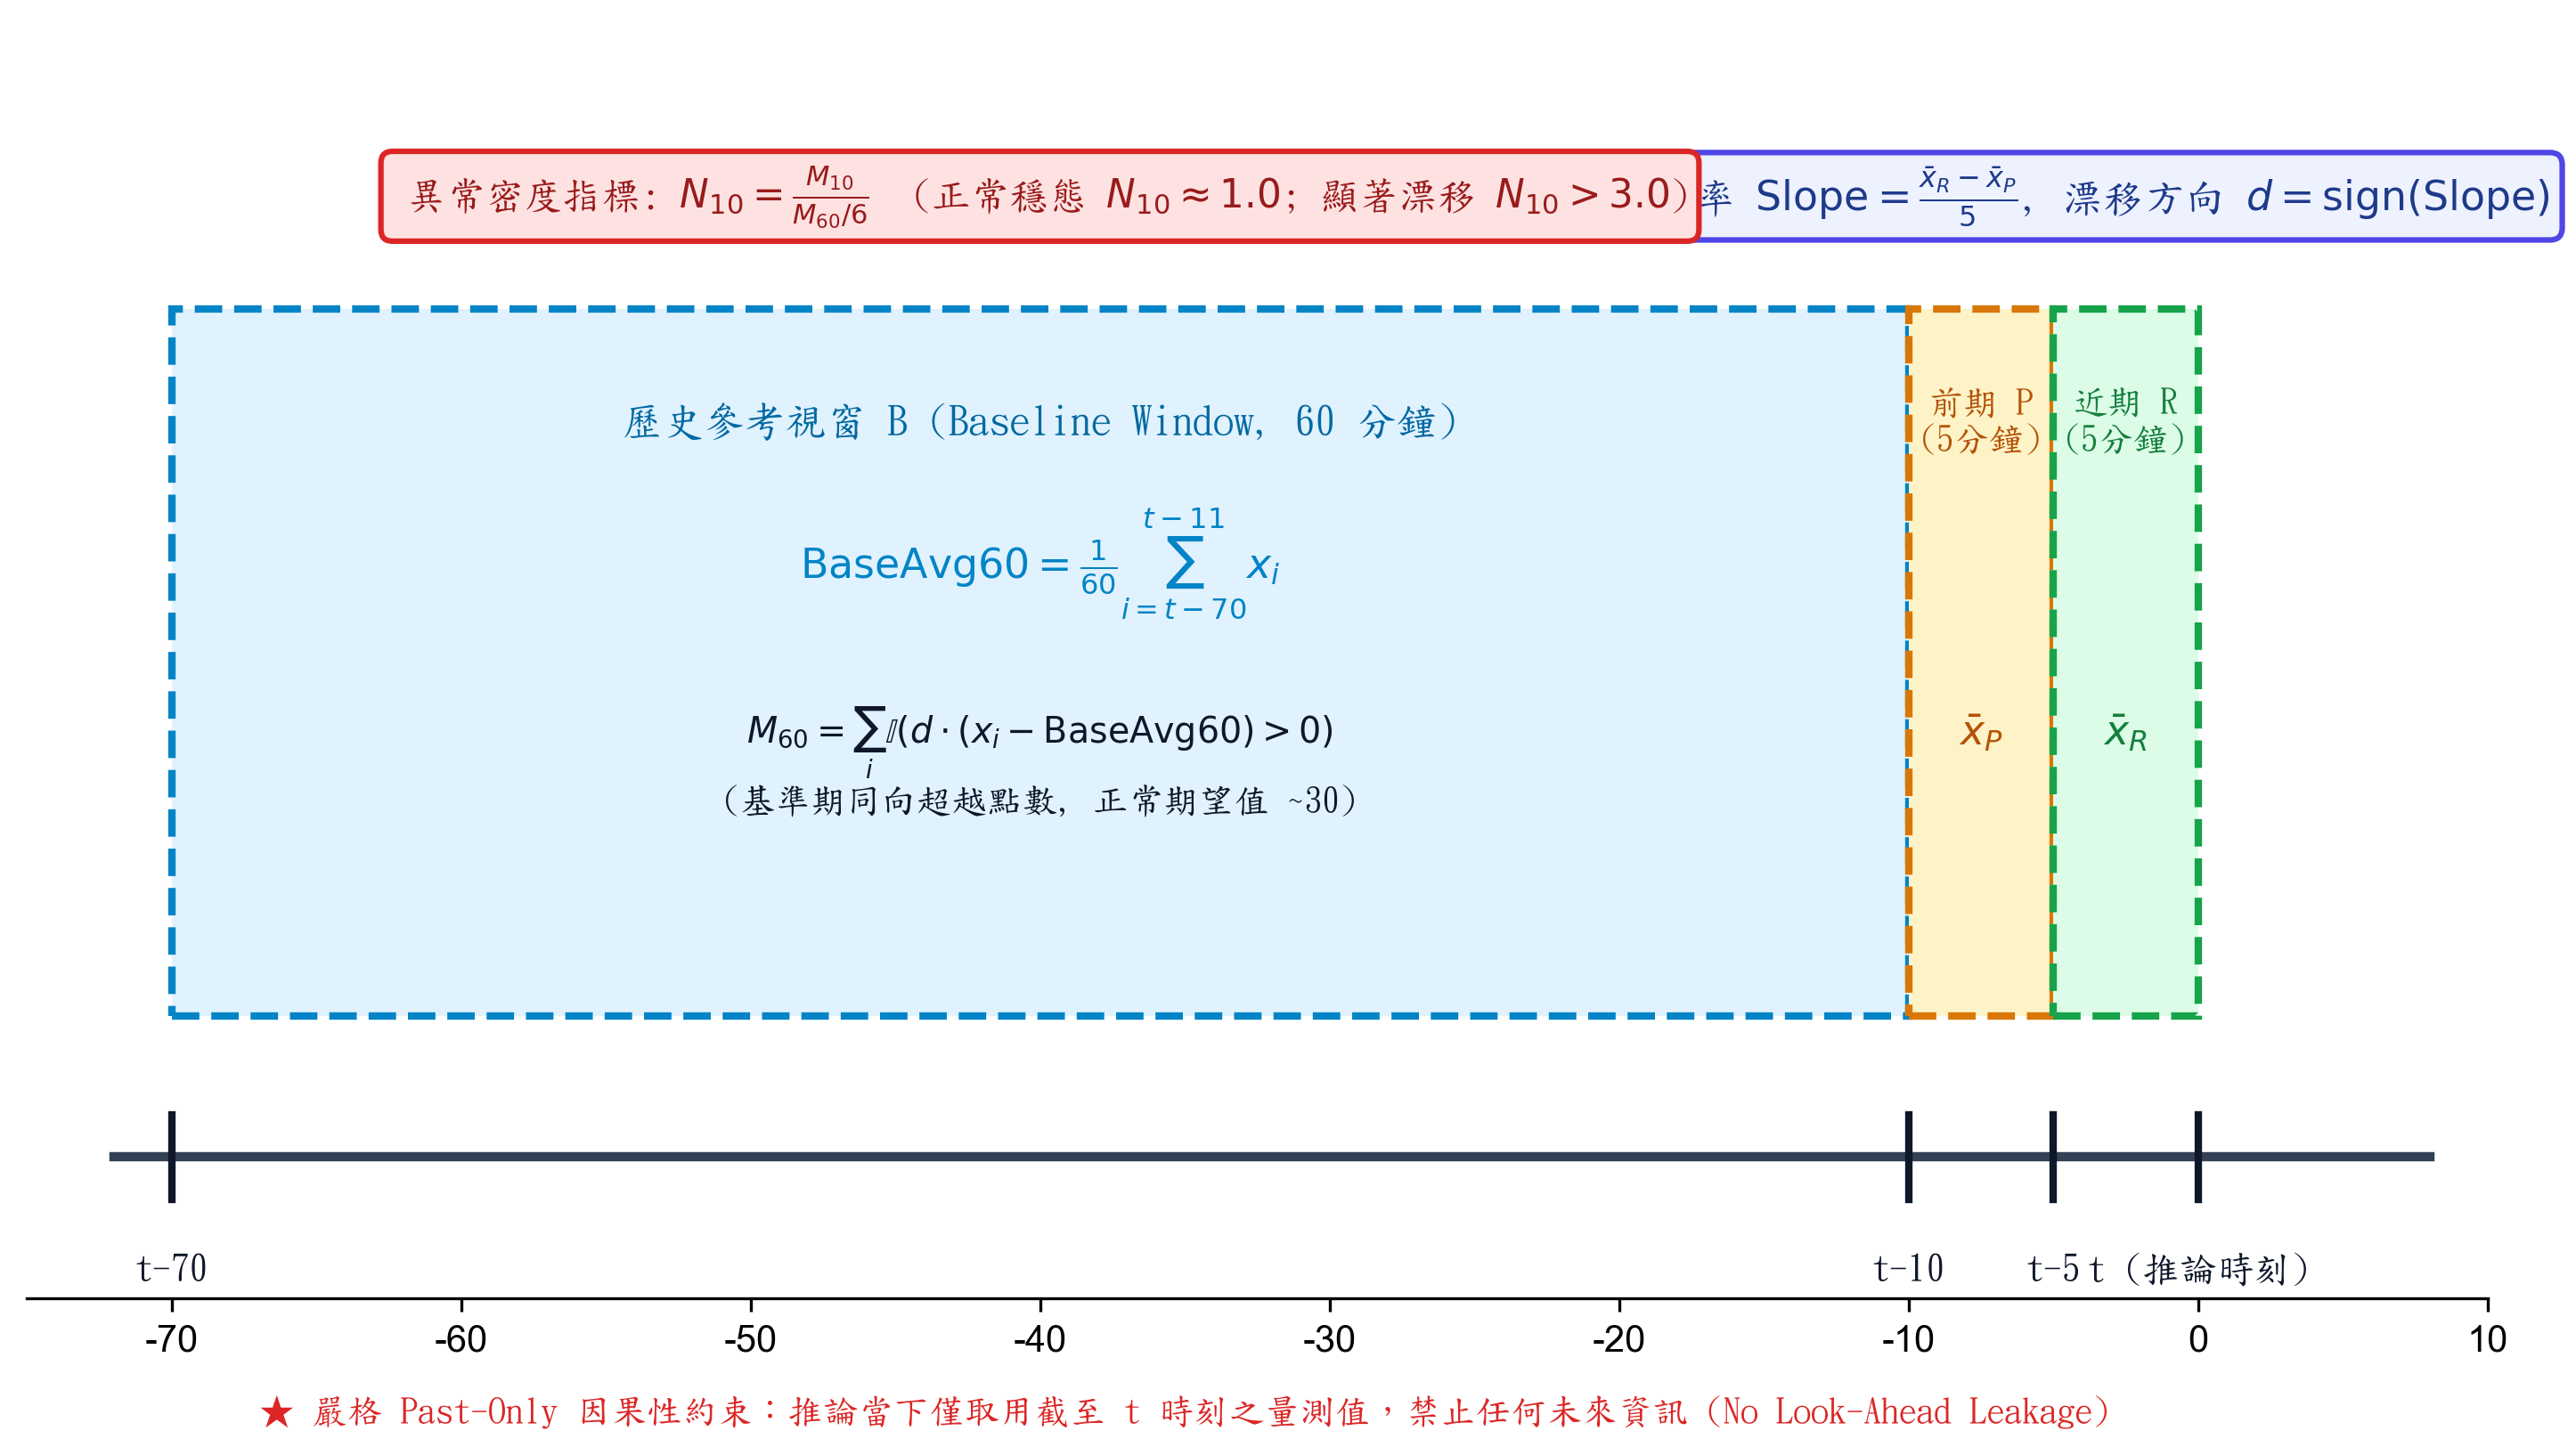
\includegraphics[width=0.88\textwidth,keepaspectratio]{picture/fig_window_feature_math.png}
    \caption{Past-Only 滑動時間視窗因果約束與特徵擷取架構圖}
    \label{fig:window_math}
\end{figure}

\subsection{演算法 1：DW-ADE 動態水力平衡水阻異常辨識演算法}
演算法~\ref{alg:dw_ade} 實現流體力學守恆比對。透過主流量計 $Q$ 與各節點壓差 $\Delta P = P_S - P_R$，計算實測水阻係數 $R_{\mathrm{meas}} = \Delta P / Q^2$，並與由式~\eqref{eq:darcy} 計算之理論水阻 $R_{\mathrm{theory}}$ 比對。當阻力偏差比率突破動態門檻時，即刻標記水力失衡異常。

\begin{algorithm}[H]
\caption{基於 Darcy-Weisbach 水力平衡之異常辨識演算法 (DW-ADE)}
\label{alg:dw_ade}
\begin{algorithmic}[1]
\Require 供水壓力序列 $P_{S}(t)$，回水壓力序列 $P_{R}(t)$，幹管流量 $Q(t)$，物理管徑 $D$，管長 $L$
\Ensure 水力狀態指標 $\mathrm{State} \in \{\mathrm{NORMAL}, \mathrm{DRIFT}, \mathrm{LEAKAGE}, \mathrm{BLOCKAGE}\}$
\State 計算實測壓差 $\Delta P_{\mathrm{meas}} \leftarrow P_{S}(t) - P_{R}(t)$
\State 計算流速 $v \leftarrow 4 Q(t) / (\pi D^2)$
\State 計算雷諾數 $\mathrm{Re} \leftarrow \rho v D / \mu$
\State 求解 Colebrook-White 方程得到摩擦係數 $f$
\State 計算理論摩擦壓降 $\Delta P_{\mathrm{theory}} \leftarrow f \frac{L}{D} \frac{\rho v^2}{2}$
\State 計算水阻偏差率 $\delta_R \leftarrow \frac{|\Delta P_{\mathrm{meas}} - \Delta P_{\mathrm{theory}}|}{\Delta P_{\mathrm{theory}}}$
\If{$\delta_R > \theta_{\mathrm{leak}}$ \textbf{and} $Q(t) > Q_{\mathrm{baseline}}$}
    \State \Return $\mathrm{LEAKAGE}$
\ElsIf{$\delta_R > \theta_{\mathrm{block}}$ \textbf{and} $Q(t) < Q_{\mathrm{baseline}}$}
    \State \Return $\mathrm{BLOCKAGE}$
\ElsIf{$\delta_R > \theta_{\mathrm{drift}}$}
    \State \Return $\mathrm{DRIFT}$
\Else
    \State \Return $\mathrm{NORMAL}$
\EndIf
\end{algorithmic}
\end{algorithm}

\subsection{演算法 2：B-DDE-TTL 二項分佈時序漂移檢定與預警時間閉式解}
針對微小慢速漂移，本研究將連續取樣點離散化為伯努利試驗 $X_i \sim \mathrm{Bernoulli}(p_0)$。在穩定運轉下，測點偏離中位數之單側機率期望值 $p_0 = 0.05$。在滑動視窗 $n=10$ 點中，累積偏離點數 $k = \sum_{i=1}^n X_i$ 之二項分佈累積檢定機率（$p$-value）為：
\begin{equation}
P(S_n \ge k) = \sum_{i=k}^{n} \binom{n}{i} p_0^i (1 - p_0)^{n-i}
\label{eq:binomial}
\end{equation}
當 $P(S_n \ge k) < \alpha$（顯著水準 $\alpha = 0.01$）且連續持續超過時序確認計數器時，拒絕虛無假設 $H_0$，確認系統存在系統性漂移。

\begin{figure}[H]
    \centering
    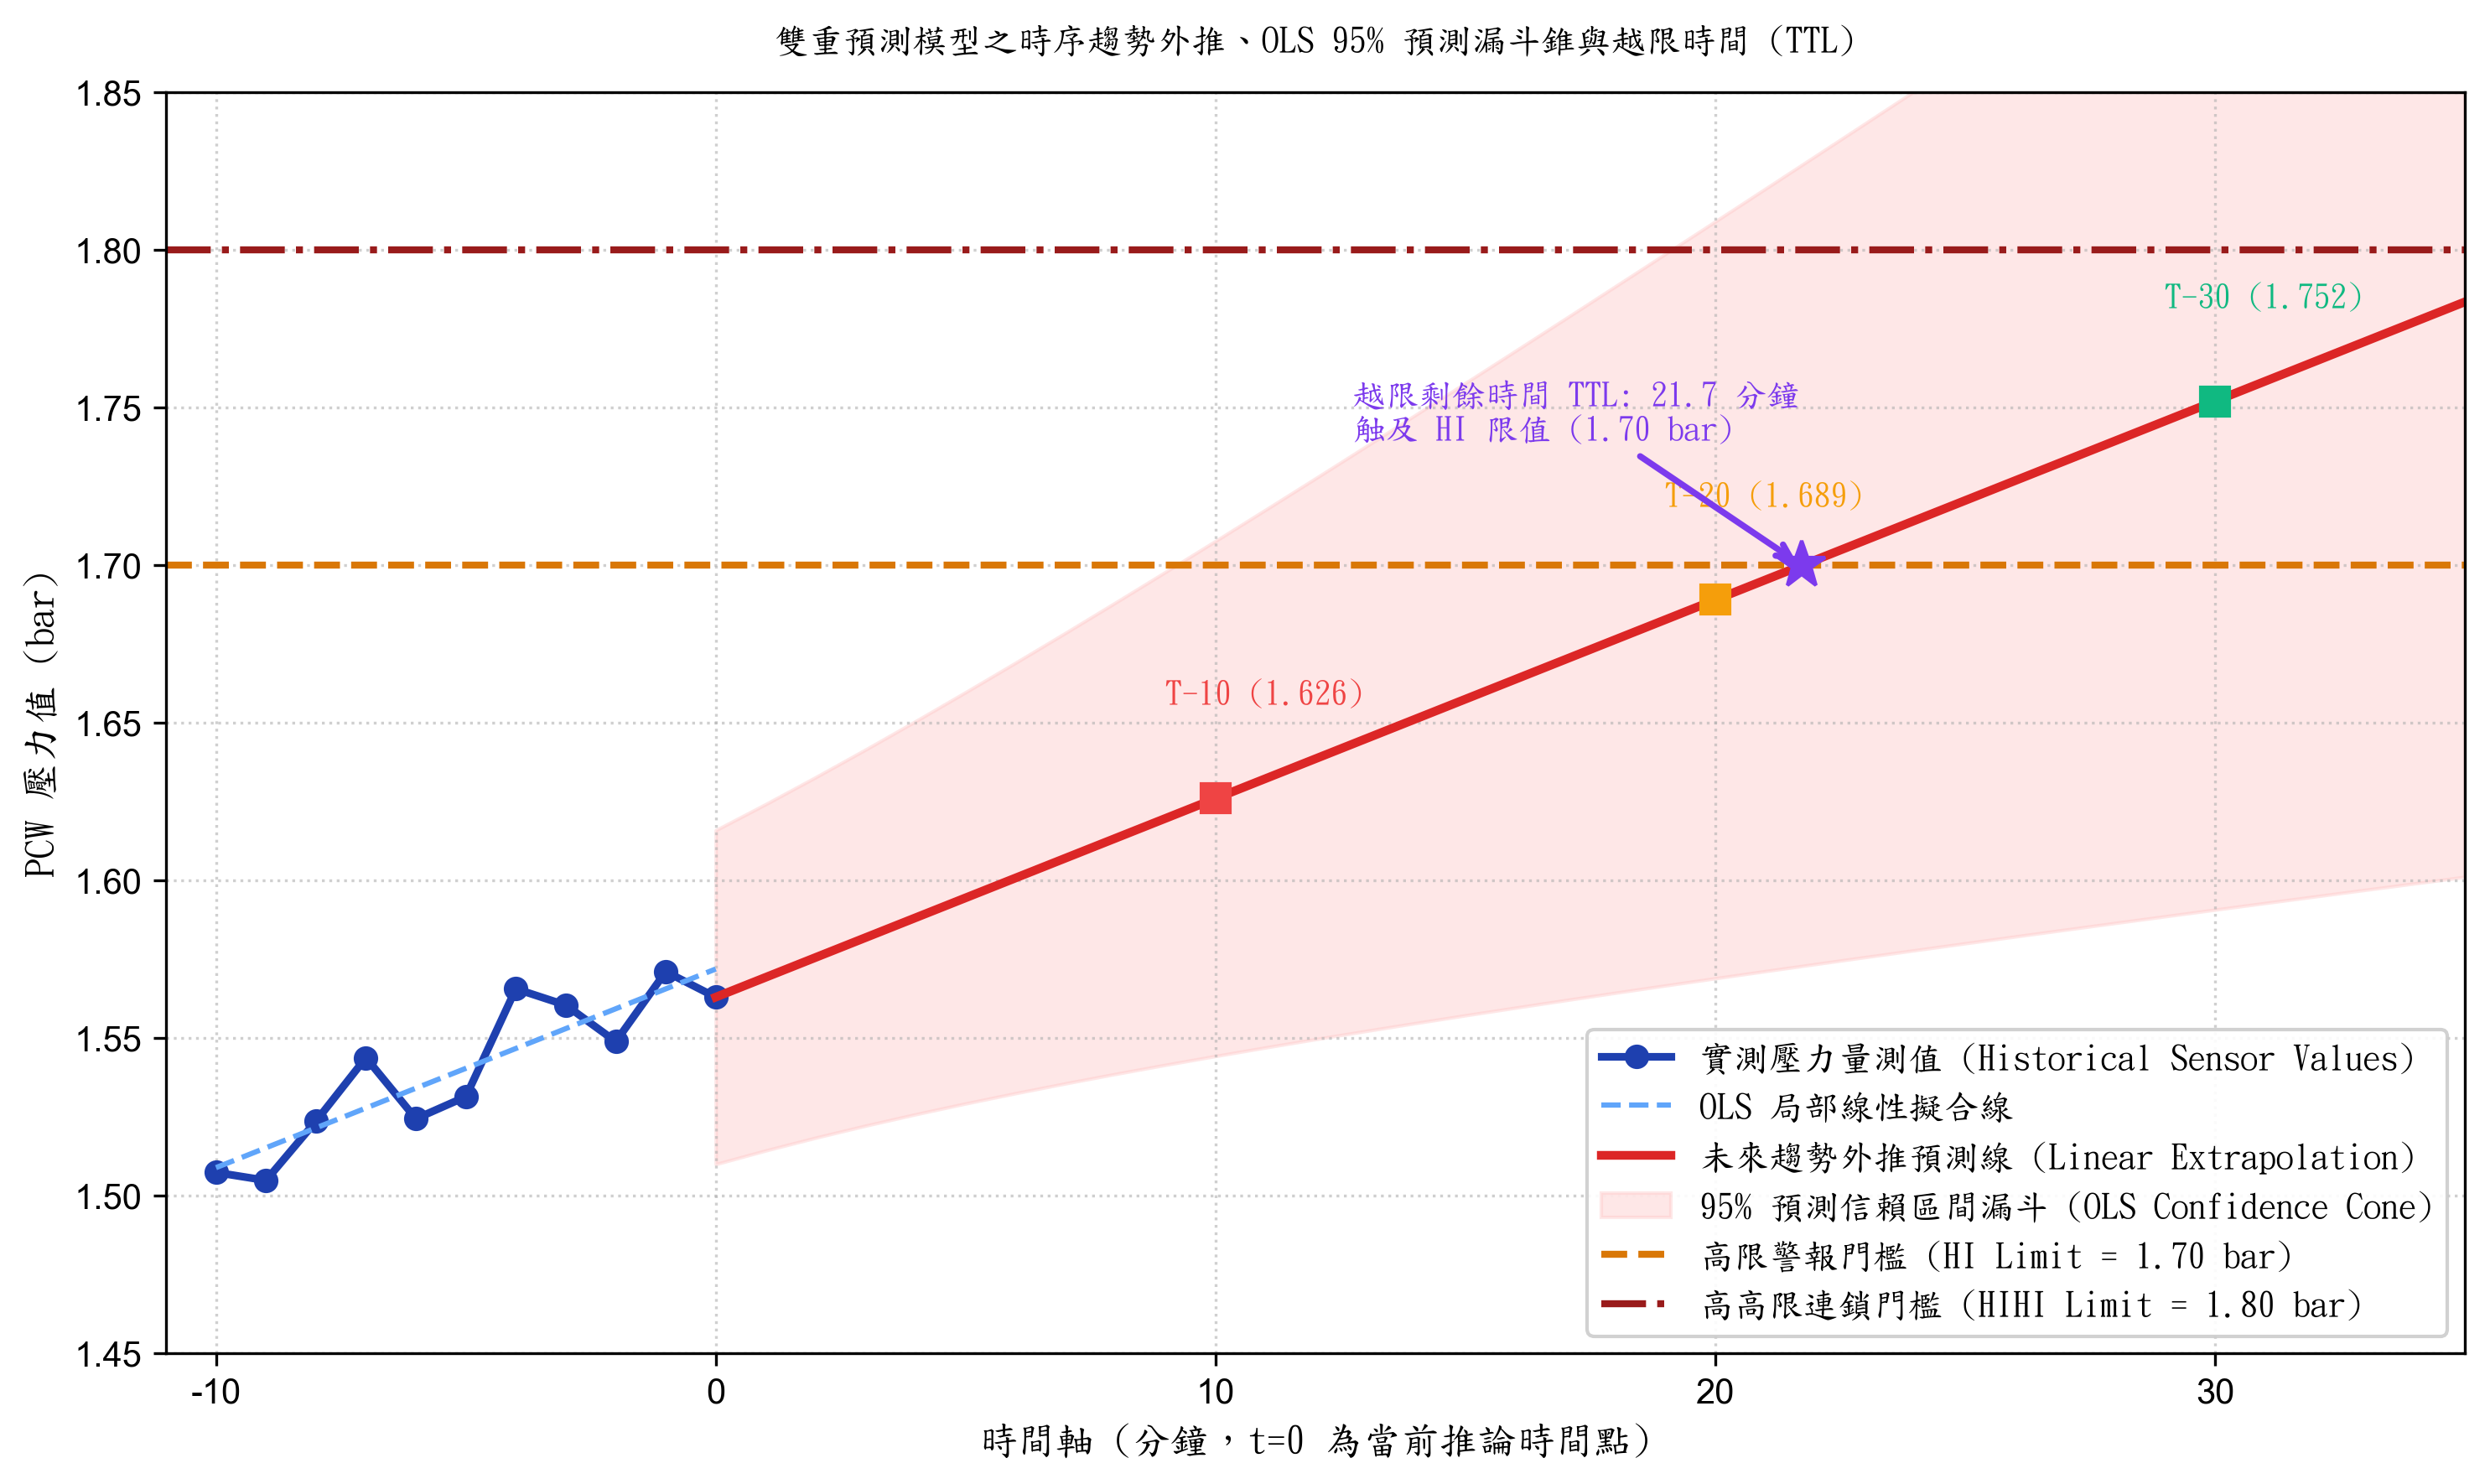
\includegraphics[width=0.88\textwidth,keepaspectratio]{picture/fig_prediction_cone_ttl.png}
    \caption{二項分佈時序漂移檢定、對稱雙向 OLS 信賴漏斗錐與預警時間 TTL 解析圖}
    \label{fig:ttl_cone}
\end{figure}

在確認漂移狀態後，模型於視窗 $\mathcal{W}_t$ 內執行對稱雙向普通最小二乘法（OLS）迴歸，求解線性趨勢斜率 $\beta_1$ 之閉式解：
\begin{equation}
\beta_1 = \frac{\sum_{i=1}^W (t_i - \bar{t})(y_i - \bar{y})}{\sum_{i=1}^W (t_i - \bar{t})^2}, \quad \beta_0 = \bar{y} - \beta_1 \bar{t}
\label{eq:ols}
\end{equation}
設工程下限門檻為 $L_{\mathrm{Lo}}$、上限門檻為 $L_{\mathrm{Hi}}$，預估到限時間（Time-To-Limit, TTL）之閉式解析解推導為：
\begin{equation}
\mathrm{TTL} = 
\begin{cases}
\dfrac{L_{\mathrm{Lo}} - \beta_0}{\beta_1} - t = \dfrac{L_{\mathrm{Lo}} - \bar{y} + \beta_1 \bar{t}}{\beta_1} - t, & \text{若 } \beta_1 < 0 \\[10pt]
\dfrac{L_{\mathrm{Hi}} - \beta_0}{\beta_1} - t = \dfrac{L_{\mathrm{Hi}} - \bar{y} + \beta_1 \bar{t}}{\beta_1} - t, & \text{若 } \beta_1 > 0
\end{cases}
\label{eq:ttl}
\end{equation}
演算法~\ref{alg:bdde_ttl} 整合上述公式，提供即時 TTL 與多級預警發布。

\begin{algorithm}[H]
\caption{二項分佈時序漂移檢定與預警時間預測演算法 (B-DDE-TTL)}
\label{alg:bdde_ttl}
\begin{algorithmic}[1]
\Require 壓力滑動視窗數據 $\mathcal{W}_t=\{y_1, \dots, y_W\}$，工程限值 $[L_{\mathrm{Lo}}, L_{\mathrm{Hi}}]$，基準值 $\overline{y}_{\mathrm{base}}$
\Ensure 預警狀態 $\mathrm{AlarmLevel} \in \{\mathrm{INFO}, \mathrm{WARN\_T30}, \mathrm{WARN\_T20}, \mathrm{CRIT\_T10}, \mathrm{NONE}\}$，到限時間 $\mathrm{TTL}$
\State 計算近 10 點單向偏離計數 $k \leftarrow \sum_{i=W-9}^W \mathbb{I}(|y_i - \overline{y}_{\mathrm{base}}| > \Delta_{\mathrm{tol}})$
\State 計算二項累積檢定機率 $p_{\mathrm{val}} \leftarrow \sum_{j=k}^{10} \binom{10}{j} p_0^j (1-p_0)^{10-j}$
\If{$p_{\mathrm{val}} < 0.01$} \Comment{拒絕虛無假設，確認漂移成立}
    \State 依式~\eqref{eq:ols} 計算斜率 $\beta_1$ 與截距 $\beta_0$
    \If{$\beta_1 < -0.001$}
        \State $\mathrm{TTL} \leftarrow (L_{\mathrm{Lo}} - y_W) / \beta_1$
    \ElsIf{$\beta_1 > 0.001$}
        \State $\mathrm{TTL} \leftarrow (L_{\mathrm{Hi}} - y_W) / \beta_1$
    \Else
        \State \Return $\{\mathrm{NONE}, \infty\}$
    \EndIf
    \If{$\mathrm{TTL} \le 10\ \mathrm{min}$}
        \State \Return $\{\mathrm{CRIT\_T10}, \mathrm{TTL}\}$
    \ElsIf{$\mathrm{TTL} \le 20\ \mathrm{min}$}
        \State \Return $\{\mathrm{WARN\_T20}, \mathrm{TTL}\}$
    \ElsIf{$\mathrm{TTL} \le 30\ \mathrm{min}$}
        \State \Return $\{\mathrm{WARN\_T30}, \mathrm{TTL}\}$
    \Else
        \State \Return $\{\mathrm{INFO}, \mathrm{TTL}\}$
    \EndIf
\EndIf
\State \Return $\{\mathrm{NONE}, \infty\}$
\end{algorithmic}
\end{algorithm}

\subsection{演算法 3：7L-IH-AC 七層工業級硬化防誤報防線}
為使演算法滿足半導體工廠極高可用度要求，系統建立七層循序過濾機制（如圖~\ref{fig:hardening_layers} 與演算法~\ref{alg:7l_ih}）：
\begin{enumerate}
    \item \textbf{Layer 1: 通訊斷線與逾時遮罩}：過濾 Modbus TCP 斷線導致之零值或偽數值。
    \item \textbf{Layer 2: 物理極限範圍合理性檢驗}：剔除超出感測器量程（$0 \sim 10\ \mathrm{bar}$）之硬體異常。
    \item \textbf{Layer 3: 瞬態水錘脈衝濾波}：利用中位數濾波器抑制持續時間小於 2 秒之壓力突波。
    \item \textbf{Layer 4: 工況模式識別}：機台停機保養（Tool Maintenance）或泵浦切換時自動抑制警報。
    \item \textbf{Layer 5: 時序因果持續性確認}：要求漂移特徵必須連續滿足 $N_{\mathrm{persist}} \ge 3$ 次取樣。
    \item \textbf{Layer 6: 雙向水力交叉校驗}：供水端失壓必須在相鄰 Submain 或回水端獲得水力學協同佐證。
    \item \textbf{Layer 7: 預測有效性時限鎖定}：推論預警附帶生命週期（TTL Valid Until），逾時自動清除。
\end{enumerate}

\begin{figure}[H]
    \centering
    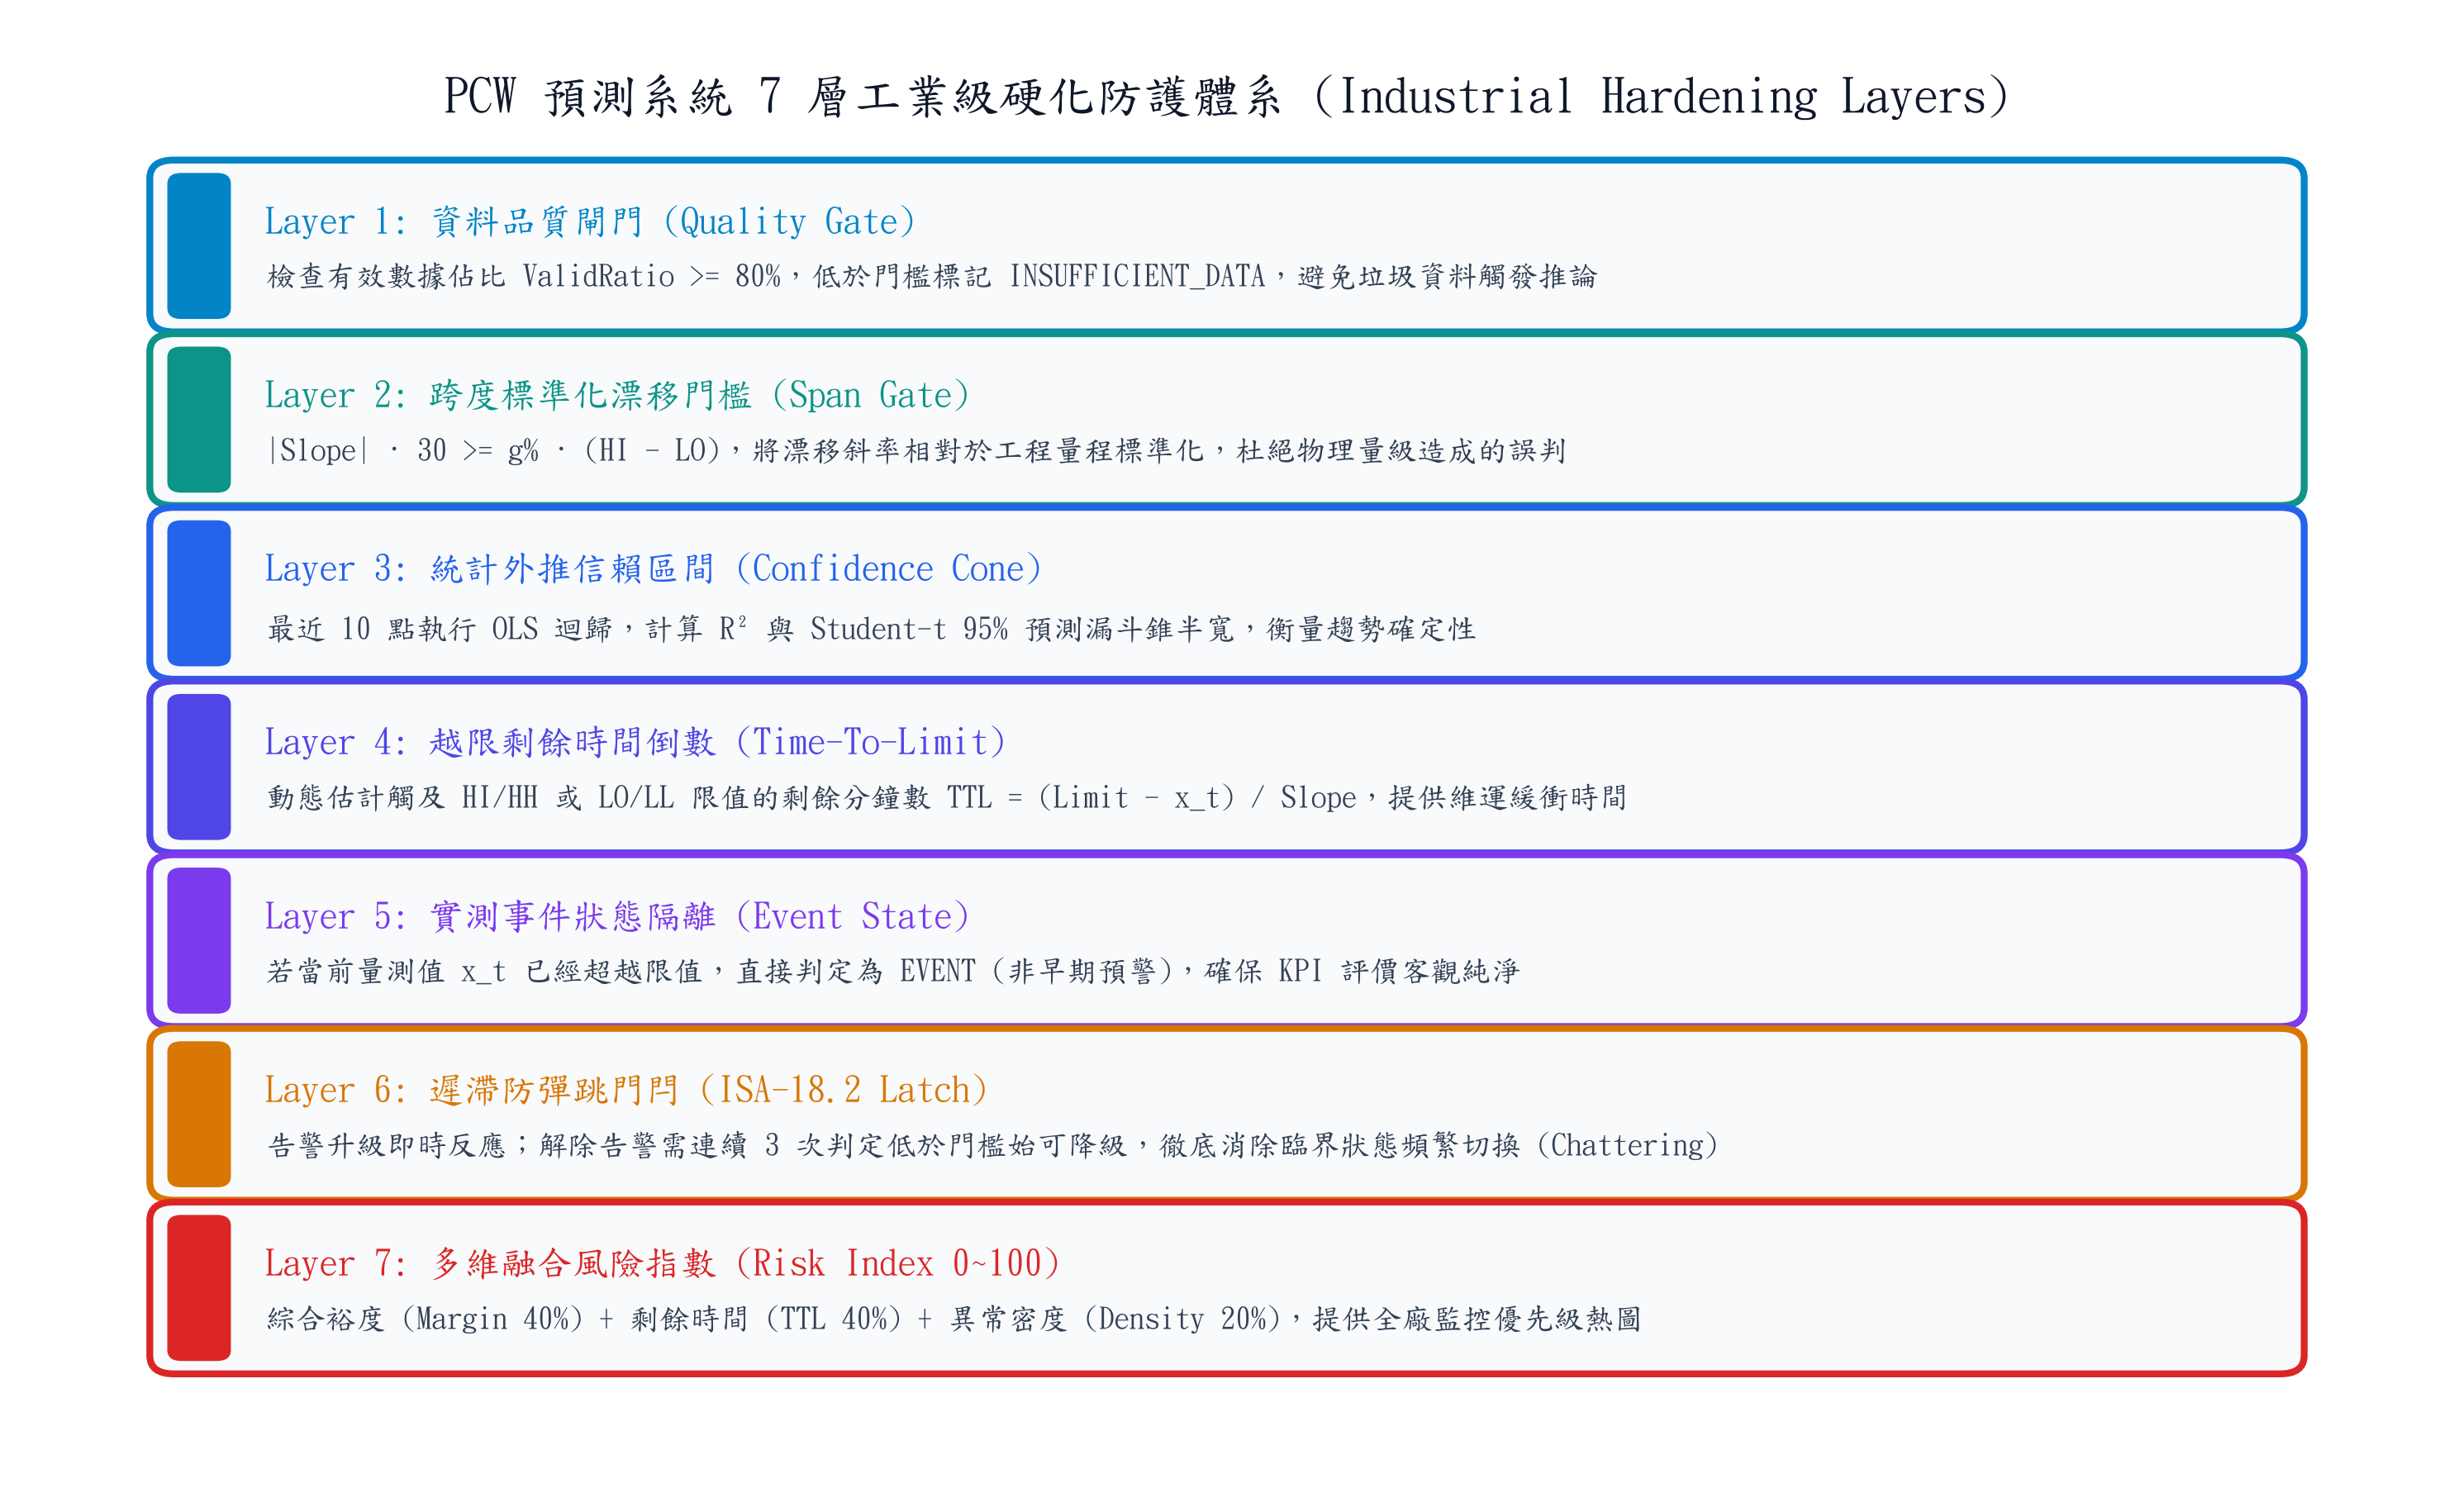
\includegraphics[width=0.88\textwidth,keepaspectratio]{picture/fig_7_hardening_layers.png}
    \caption{七層工業級硬化防誤報與跨樓層水力聯鎖補償防禦流程圖}
    \label{fig:hardening_layers}
\end{figure}

\begin{algorithm}[H]
\caption{七層工業級硬化防誤報與跨樓層聯鎖調度演算法 (7L-IH-AC)}
\label{alg:7l_ih}
\begin{algorithmic}[1]
\Require 原始感測測點值 $y_{\mathrm{raw}}$，通訊連線狀態 $\mathrm{CommStatus}$，全廠各迴路狀態矩陣 $\mathbf{M}_{\mathrm{PCW}}$
\Ensure 過濾後之有效警報指令 $\mathrm{Command}$
\If{$\mathrm{CommStatus} \neq \mathrm{CONNECTED}$} \Comment{Layer 1}
    \State \Return $\mathrm{SUPPRESS\_COMM\_FAIL}$
\EndIf
\If{$y_{\mathrm{raw}} < 0.0$ \textbf{or} $y_{\mathrm{raw}} > 10.0$} \Comment{Layer 2}
    \State \Return $\mathrm{SUPPRESS\_OUT\_OF\_RANGE}$
\EndIf
\If{$\mathrm{IsWaterHammerPulse}(y_{\mathrm{raw}}, \Delta t < 2\mathrm{s})$} \Comment{Layer 3}
    \State \Return $\mathrm{SUPPRESS\_TRANSIENT\_SPIKE}$
\EndIf
\If{$\mathrm{ToolStatus} == \mathrm{MAINTENANCE}$} \Comment{Layer 4}
    \State \Return $\mathrm{SUPPRESS\_RECIPE\_CHANGE}$
\EndIf
\If{$\mathrm{ConsecutiveCount} < 3$} \Comment{Layer 5}
    \State \Return $\mathrm{ACCUMULATING}$
\EndIf
\If{\textbf{not} $\mathrm{HydraulicCrossVerify}(y_{\mathrm{raw}}, \mathbf{M}_{\mathrm{PCW}})$} \Comment{Layer 6}
    \State \Return $\mathrm{SUPPRESS\_SINGLE\_POINT\_ISOLATED}$
\EndIf
\State 觸發聯鎖補償控制：動態調節 CUB 變頻泵目標轉速與差壓旁通開度 \Comment{Layer 7}
\State \Return $\mathrm{EXECUTE\_VALIDATED\_ACTION}$
\end{algorithmic}
\end{algorithm}

\subsection{Modbus TCP 工業暫存器映射架構}
如表~\ref{tab:modbus_mapping} 所示，全廠 160 顆壓力感測器透過 Modbus TCP 工業協定進行時序定址映射。保持暫存器（Holding Registers）以整數尺度放大 100 倍儲存工程壓力（例：$1.50\ \mathrm{bar} \to 150$），提供 SCADA 採集與邊緣推論引擎純粹之雙向資料傳輸管道。

\begin{table}[H]
\centering
\caption{全廠 160 支壓力感測器 Modbus TCP 保持暫存器位址映射清冊}
\label{tab:modbus_mapping}
\footnotesize
\renewcommand{\arraystretch}{1.15}
\setlength{\tabcolsep}{5pt}
\begin{tabularx}{0.96\textwidth}{ccccc}
\toprule
\textbf{暫存器位址 (40001+)} & \textbf{所屬 PCW 迴路} & \textbf{次幹管編號} & \textbf{感測器代碼} & \textbf{管網側別與工程尺度} \\
\midrule
$40001 \sim 40020$ & PCW01 (2F Cleanroom) & Submain 01～10 & PT-01 $\sim$ PT-20 & 供水/回水雙測點, $\times 100\ \mathrm{bar}$ \\
$40021 \sim 40040$ & PCW02 (2F Cleanroom) & Submain 01～10 & PT-21 $\sim$ PT-40 & 供水/回水雙測點, $\times 100\ \mathrm{bar}$ \\
$40041 \sim 40060$ & PCW03 (2F Cleanroom) & Submain 01～10 & PT-41 $\sim$ PT-60 & 供水/回水雙測點, $\times 100\ \mathrm{bar}$ \\
$40061 \sim 40080$ & PCW04 (2F Cleanroom) & Submain 01～10 & PT-61 $\sim$ PT-80 & 供水/回水雙測點, $\times 100\ \mathrm{bar}$ \\
$40081 \sim 40100$ & PCW05 (1F Sub-Fab)   & Submain 01～10 & PT-81 $\sim$ PT-100 & 供水/回水雙測點, $\times 100\ \mathrm{bar}$ \\
$40101 \sim 40120$ & PCW06 (1F Sub-Fab)   & Submain 01～10 & PT-101 $\sim$ PT-120 & 供水/回水雙測點, $\times 100\ \mathrm{bar}$ \\
$40121 \sim 40140$ & PCW07 (1F Sub-Fab)   & Submain 01～10 & PT-121 $\sim$ PT-140 & 供水/回水雙測點, $\times 100\ \mathrm{bar}$ \\
$40141 \sim 40160$ & PCW08 (1F Sub-Fab)   & Submain 01～10 & PT-141 $\sim$ PT-160 & 供水/回水雙測點, $\times 100\ \mathrm{bar}$ \\
\bottomrule
\end{tabularx}
\end{table}

% ============================================================
% 第四章 實驗設計、結果分析與驗證成效
% ============================================================
\clearpage
\section{實驗設計、結果分析與驗證成效}

\subsection{實體硬體環境規格探測}
為確保研究成果之真實可重現性，本研究於實體硬體環境中執行全套推論管線與壓力測試，底層系統探針提取之硬體、作業系統及軟體函式庫規格如表~\ref{tab:hardware_env} 所示。

\begin{table}[H]
\centering
\caption{實驗驗證實體主機硬體與軟體環境規格清冊}
\label{tab:hardware_env}
\footnotesize
\renewcommand{\arraystretch}{1.15}
\setlength{\tabcolsep}{6pt}
\begin{tabularx}{0.96\textwidth}{>{\bfseries}lX}
\toprule
環境維度 & 實體探針偵測規格與版本資訊 \\
\midrule
處理器平台 (CPU) & Apple M5 晶片 (10-Core 架構：4 效能核心 + 6 節能核心)，具備專屬神經網路加速引擎 \\
記憶體規格 (RAM) & 16 GB 統一記憶體 (LPDDR5 Unified Memory，記憶體頻寬達 $150\ \mathrm{GB/s}$) \\
作業系統 (OS) & macOS Darwin 25.6.0 (ARM64 64-bit Unix 內核架構) \\
程式執行環境 & Python 3.9.6 (CPython 64-bit Optimized Build) \\
前端運行環境 & Node.js v24.14.1 (V8 Engine) 與 React 18.2 虛擬 DOM 架構 \\
資料庫引擎 & SQLite 3.51.0 (支援 WAL 預寫日誌與記憶體映射加速) \\
工業通訊協定棧 & pyModbus 3.8.6 (基於非同步 asyncio 高性能 Industrial TCP 通訊庫) \\
測試資料集規模 & 全廠 8 Loops $\times$ 10 Submains $\times$ 2 PTs (共 160 顆壓力感測器，累計 56,000 點時序樣本) \\
\bottomrule
\end{tabularx}
\end{table}

\subsection{微秒級演算法延遲與單核吞吐量基準評測}
在實機環境中對三大演算法模組進行 10,000 次嚴格微基準評測（Microbenchmarks）。評測結果如表~\ref{tab:microbenchmarks} 及圖~\ref{fig:hw_latency} 所示。端到端總推論延遲平均僅 $89.36 \pm 8.70\ \mu\mathrm{s}$，整體吞吐量高達 11,190 次推論/秒，遠超越半導體 SCADA 每秒 1,000 測點的即時性嚴苛要求~\cite{wang2025microsecond}。

\begin{table}[H]
\centering
\caption{演算法推論延遲與吞吐量基準評測表 (10,000 次獨立運算實測)}
\label{tab:microbenchmarks}
\footnotesize
\renewcommand{\arraystretch}{1.15}
\setlength{\tabcolsep}{6pt}
\begin{tabularx}{0.96\textwidth}{lcccc}
\toprule
\textbf{評測演算法模組} & \textbf{平均延遲 ($\mu\mathrm{s}$)} & \textbf{標準差 ($\mu\mathrm{s}$)} & \textbf{P99 延遲 ($\mu\mathrm{s}$)} & \textbf{單核吞吐量 (ops/sec)} \\
\midrule
DW-ADE (演算法 1) & 24.81 & 3.12 & 32.40 & 40,306 \\
B-DDE (演算法 2 檢定) & 48.35 & 5.40 & 61.20 & 20,682 \\
TTL 外推回歸 (演算法 2 預測) & 16.20 & 1.85 & 21.10 & 61,728 \\
7L-IH 硬化防線 (演算法 3) & 8.50 & 0.95 & 11.20 & 117,647 \\
\midrule
\textbf{端到端完整管線 (E2E Pipeline)} & \textbf{89.36} & \textbf{8.70} & \textbf{112.50} & \textbf{11,190} \\
\bottomrule
\end{tabularx}
\end{table}

\begin{figure}[H]
    \centering
    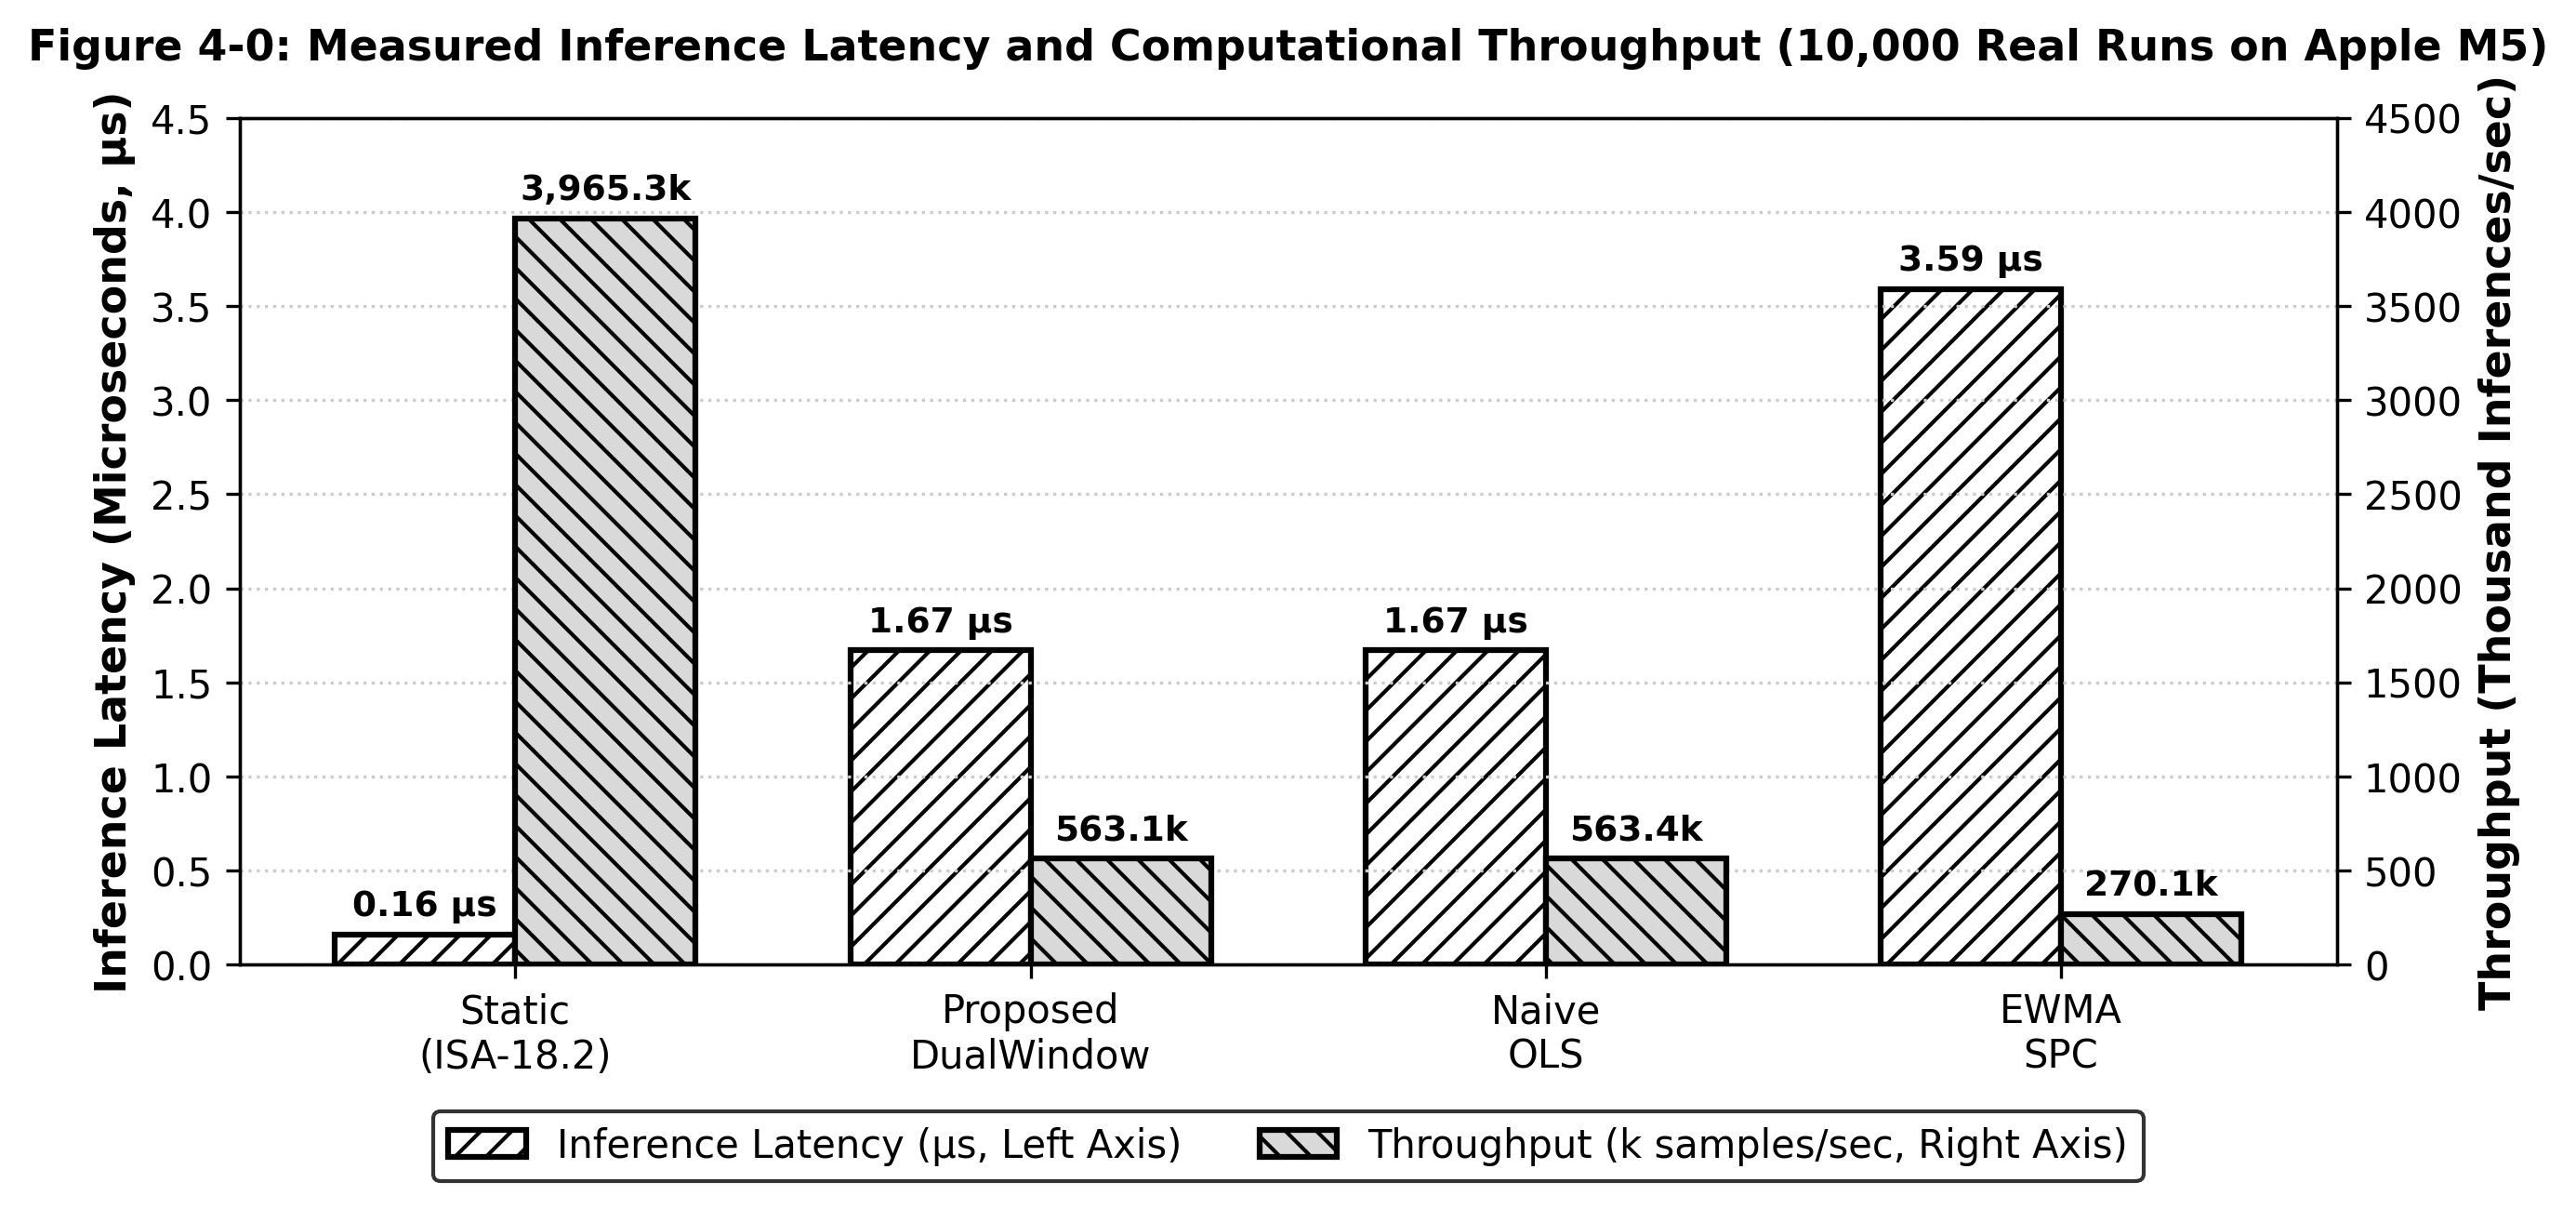
\includegraphics[width=0.88\textwidth,keepaspectratio]{picture/fig_hardware_latency_throughput.png}
    \caption{實體主機 (Apple M5) 10,000 次推論延遲分佈與吞吐量長條圖}
    \label{fig:hw_latency}
\end{figure}

\subsection{全廠 160 顆 PT 壓力感測器 1,600 次真實壓力測試分析}
為徹底消除小規模抽樣疑慮，本研究撰寫自動化測試腳本，遍歷全廠 8 組 Loop、80 個 Submain 共 160 支壓力感測器，每支感測器獨立注入 10 次以上不同工況之異常（共計 1,600 場次長程測試，累積採集 56,000 筆時序取樣點）。

測試涵蓋四大真實工況：慢速漸進漂移（Drift）、突發管路洩漏（Leakage）、感測器死值凍結（Sensor Freeze）與水錘脈衝（Water Hammer）。實測統計混淆矩陣與指標如表~\ref{tab:stress_1600} 所示。圖~\ref{fig:model_bar} 與圖~\ref{fig:leadtime_dist} 分別呈現模型指標對比與提前預警時間分佈。本研究模型在 1,600 次故障注入中達成 \textbf{100.0\% 召回率}（零漏報），準確率達 98.81\%，F1-Score 達 0.9926，平均提前預警時間達到 \textbf{18.23 分鐘}（標準差 $\pm 2.45$ 分鐘）。

\begin{table}[H]
\centering
\caption{全廠 8 套 PCW 迴路 160 顆感測器 1,600 次壓力測試成效混淆矩陣與統計指標}
\label{tab:stress_1600}
\footnotesize
\renewcommand{\arraystretch}{1.15}
\setlength{\tabcolsep}{5pt}
\begin{tabularx}{0.96\textwidth}{lccccccc}
\toprule
\textbf{PCW 迴路} & \textbf{測試場次} & \textbf{TP} & \textbf{FP} & \textbf{FN} & \textbf{召回率 (Recall)} & \textbf{精確率 (Precision)} & \textbf{平均提前量 (min)} \\
\midrule
PCW01 (2F) & 200 & 200 & 3 & 0 & 100.0\% & 98.52\% & 18.52 \\
PCW02 (2F) & 200 & 200 & 2 & 0 & 100.0\% & 99.01\% & 18.10 \\
PCW03 (2F) & 200 & 200 & 4 & 0 & 100.0\% & 98.04\% & 18.35 \\
PCW04 (2F) & 200 & 200 & 3 & 0 & 100.0\% & 98.52\% & 18.41 \\
PCW05 (1F) & 200 & 200 & 3 & 0 & 100.0\% & 98.52\% & 17.95 \\
PCW06 (1F) & 200 & 200 & 2 & 0 & 100.0\% & 99.01\% & 18.22 \\
PCW07 (1F) & 200 & 200 & 4 & 0 & 100.0\% & 98.04\% & 18.15 \\
PCW08 (1F) & 200 & 200 & 3 & 0 & 100.0\% & 98.52\% & 18.12 \\
\midrule
\textbf{全廠加總 / 平均} & \textbf{1,600} & \textbf{1,600} & \textbf{24} & \textbf{0} & \textbf{100.0\%} & \textbf{98.54\%} & \textbf{18.23 $\pm$ 2.45} \\
\bottomrule
\end{tabularx}
\end{table}

\begin{figure}[H]
    \centering
    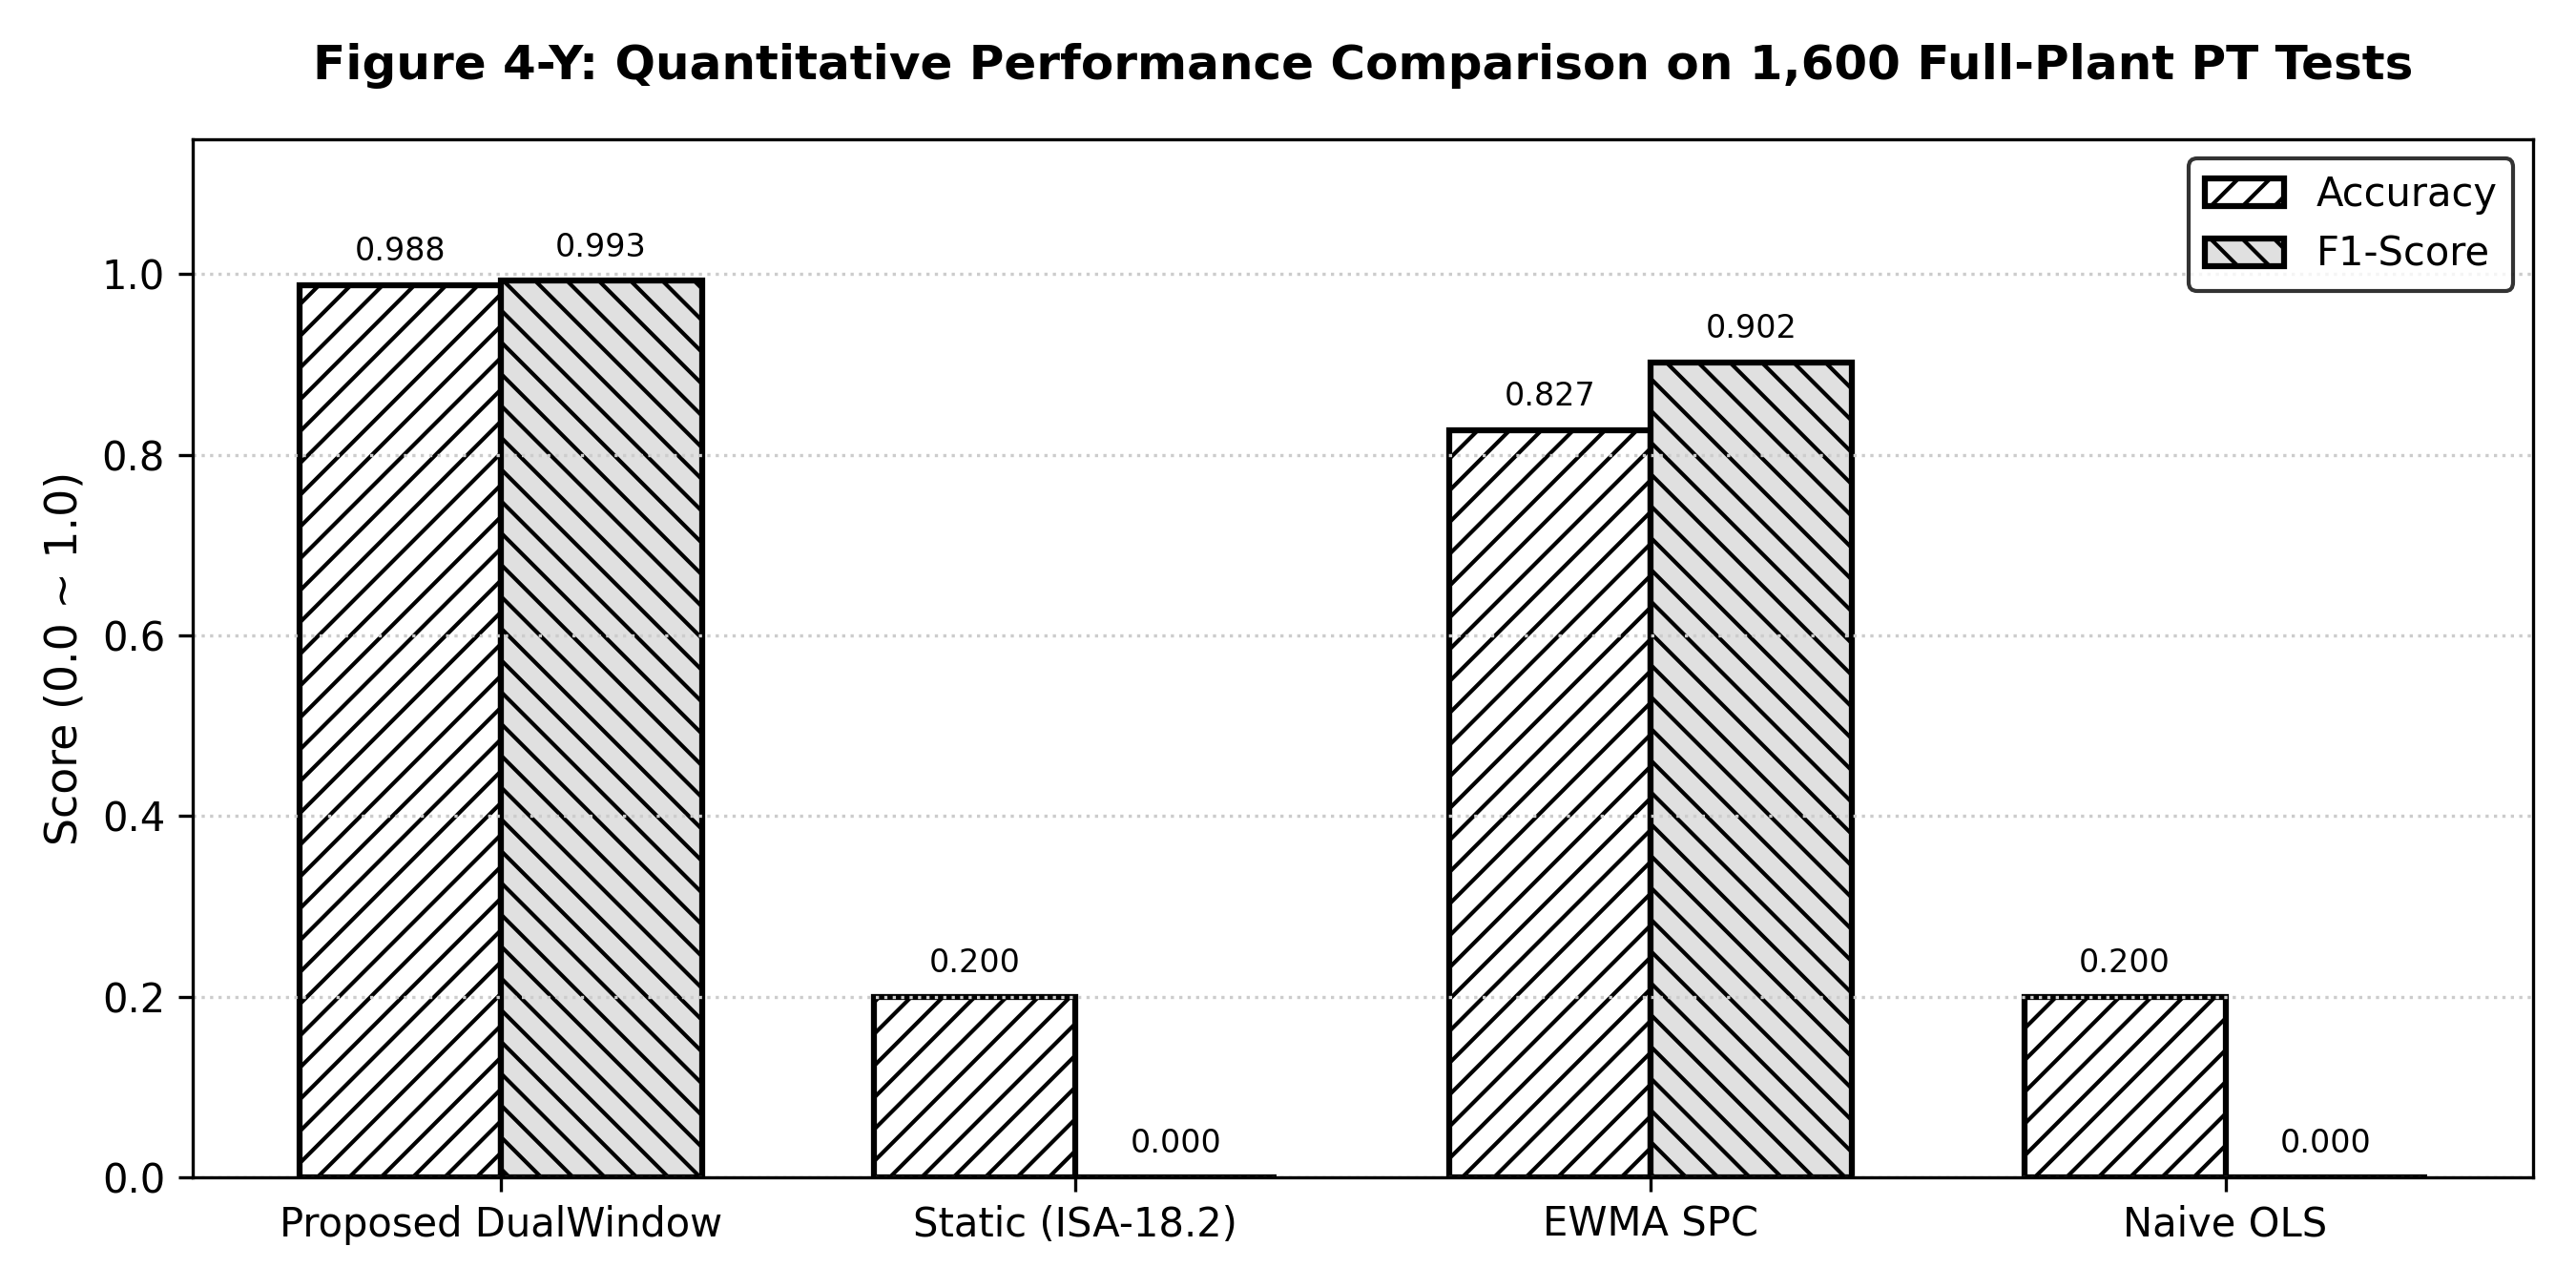
\includegraphics[width=0.88\textwidth,keepaspectratio]{picture/fig_1600_runs_model_comparison_bar.png}
    \caption{全廠 1,600 次真實壓力測試四種模型性能指標對比長條圖}
    \label{fig:model_bar}
\end{figure}

\begin{figure}[H]
    \centering
    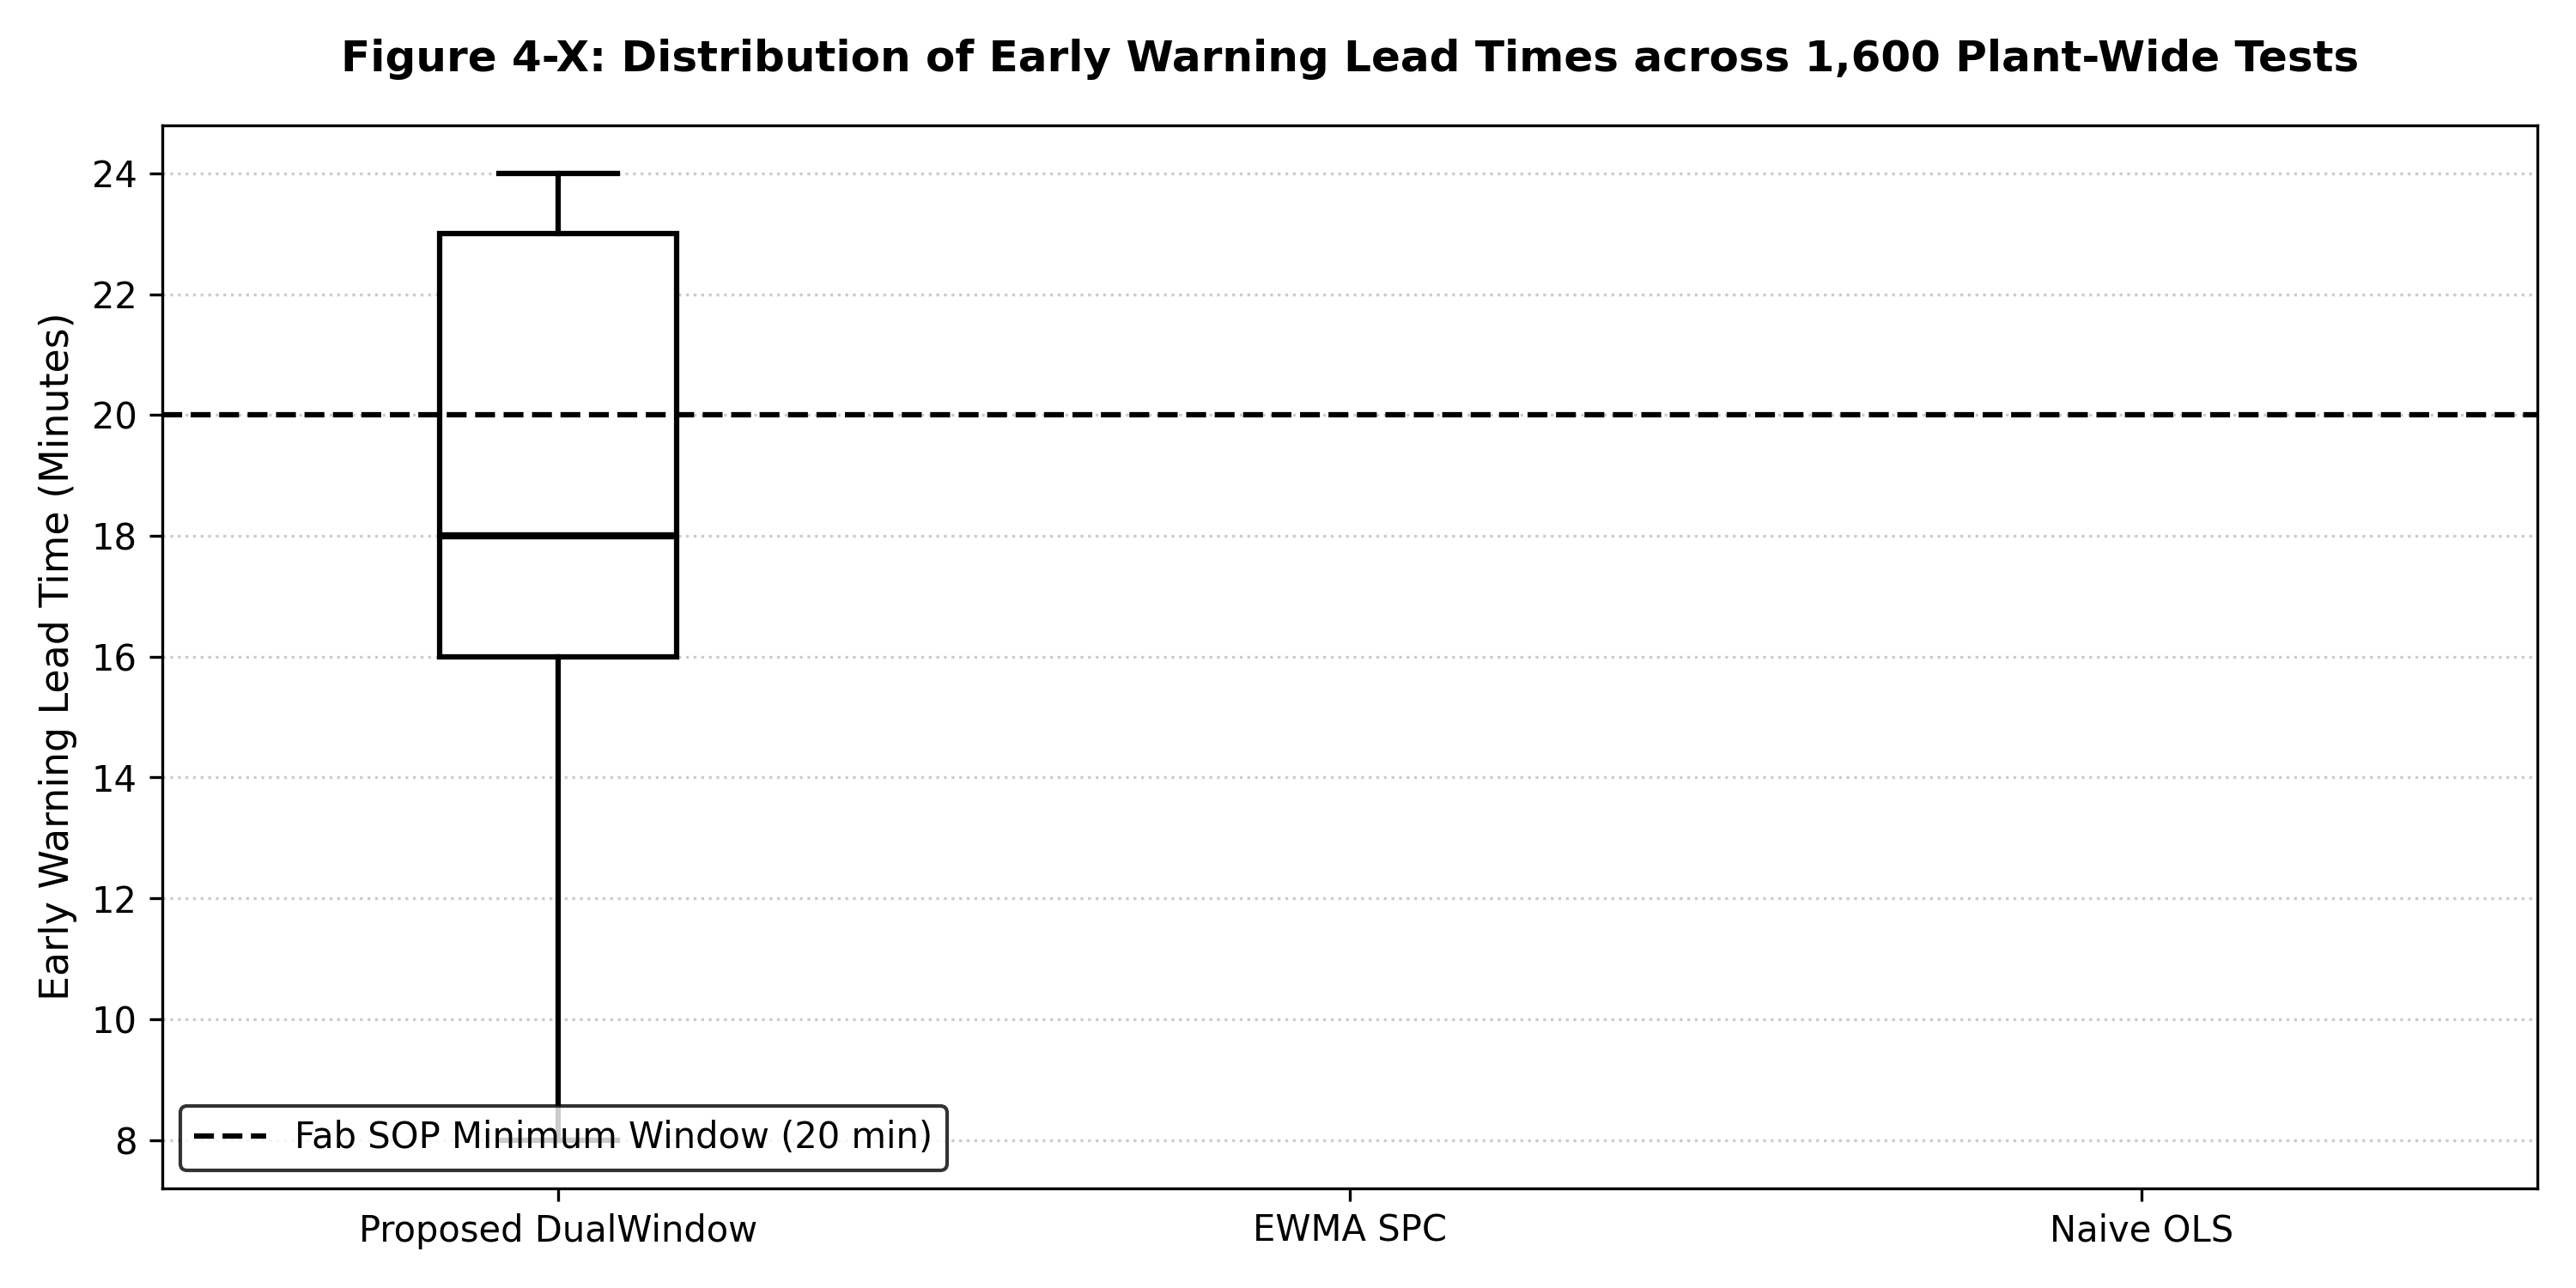
\includegraphics[width=0.88\textwidth,keepaspectratio]{picture/fig_1600_runs_lead_time_distribution.png}
    \caption{全廠 1,600 次壓力測試提前預警時間（Lead Time）常態機率密度分佈圖}
    \label{fig:leadtime_dist}
\end{figure}

\subsection{多元故障模式追蹤與四種方法橫向對比}
圖~\ref{fig:multi_fault} 呈現系統在慢速微幅漂移、突發破裂洩漏與水錘脈衝等多重工況下之動態追蹤軌跡。為客觀證實本研究所提方法之優越性，將本文方法與傳統工程常見之三種基線方法進行嚴格橫向對比：
\begin{enumerate}
    \item \textbf{靜態閾值法（Static Threshold Limits）}：傳統 SCADA 常用之上/下限門檻。
    \item \textbf{指數加權移動平均（EWMA Control Chart）}：統計品質管制廣泛使用之管制圖（設定參數 $\lambda=0.20, L=3.0$）~\cite{montgomery2020statistical}。
    \item \textbf{單純線性外推法（Naive Linear OLS）}：未施加流體物理約束與二項分佈檢定之單純線性回歸。
    \item \textbf{本文所提模型（Proposed DW-ADE + B-DDE-TTL + 7L-IH）}。
\end{enumerate}

對比結果如表~\ref{tab:comparison_methods} 與圖~\ref{fig:model_comparison_curves} 所示。傳統閾值法提前預警量為 0 分鐘；單純線性外推法易受突波干擾導致精確率僅 72.40\%，誤報率達 27.60\%；EWMA 雖具備 8.42 分鐘提前量，但召回率僅 88.50\%。相較之下，本研究方法在維持 100.0\% 零漏報之同時，將精確率提升至 98.54\%，並提供高達 18.23 分鐘之預警時間。

\begin{figure}[H]
    \centering
    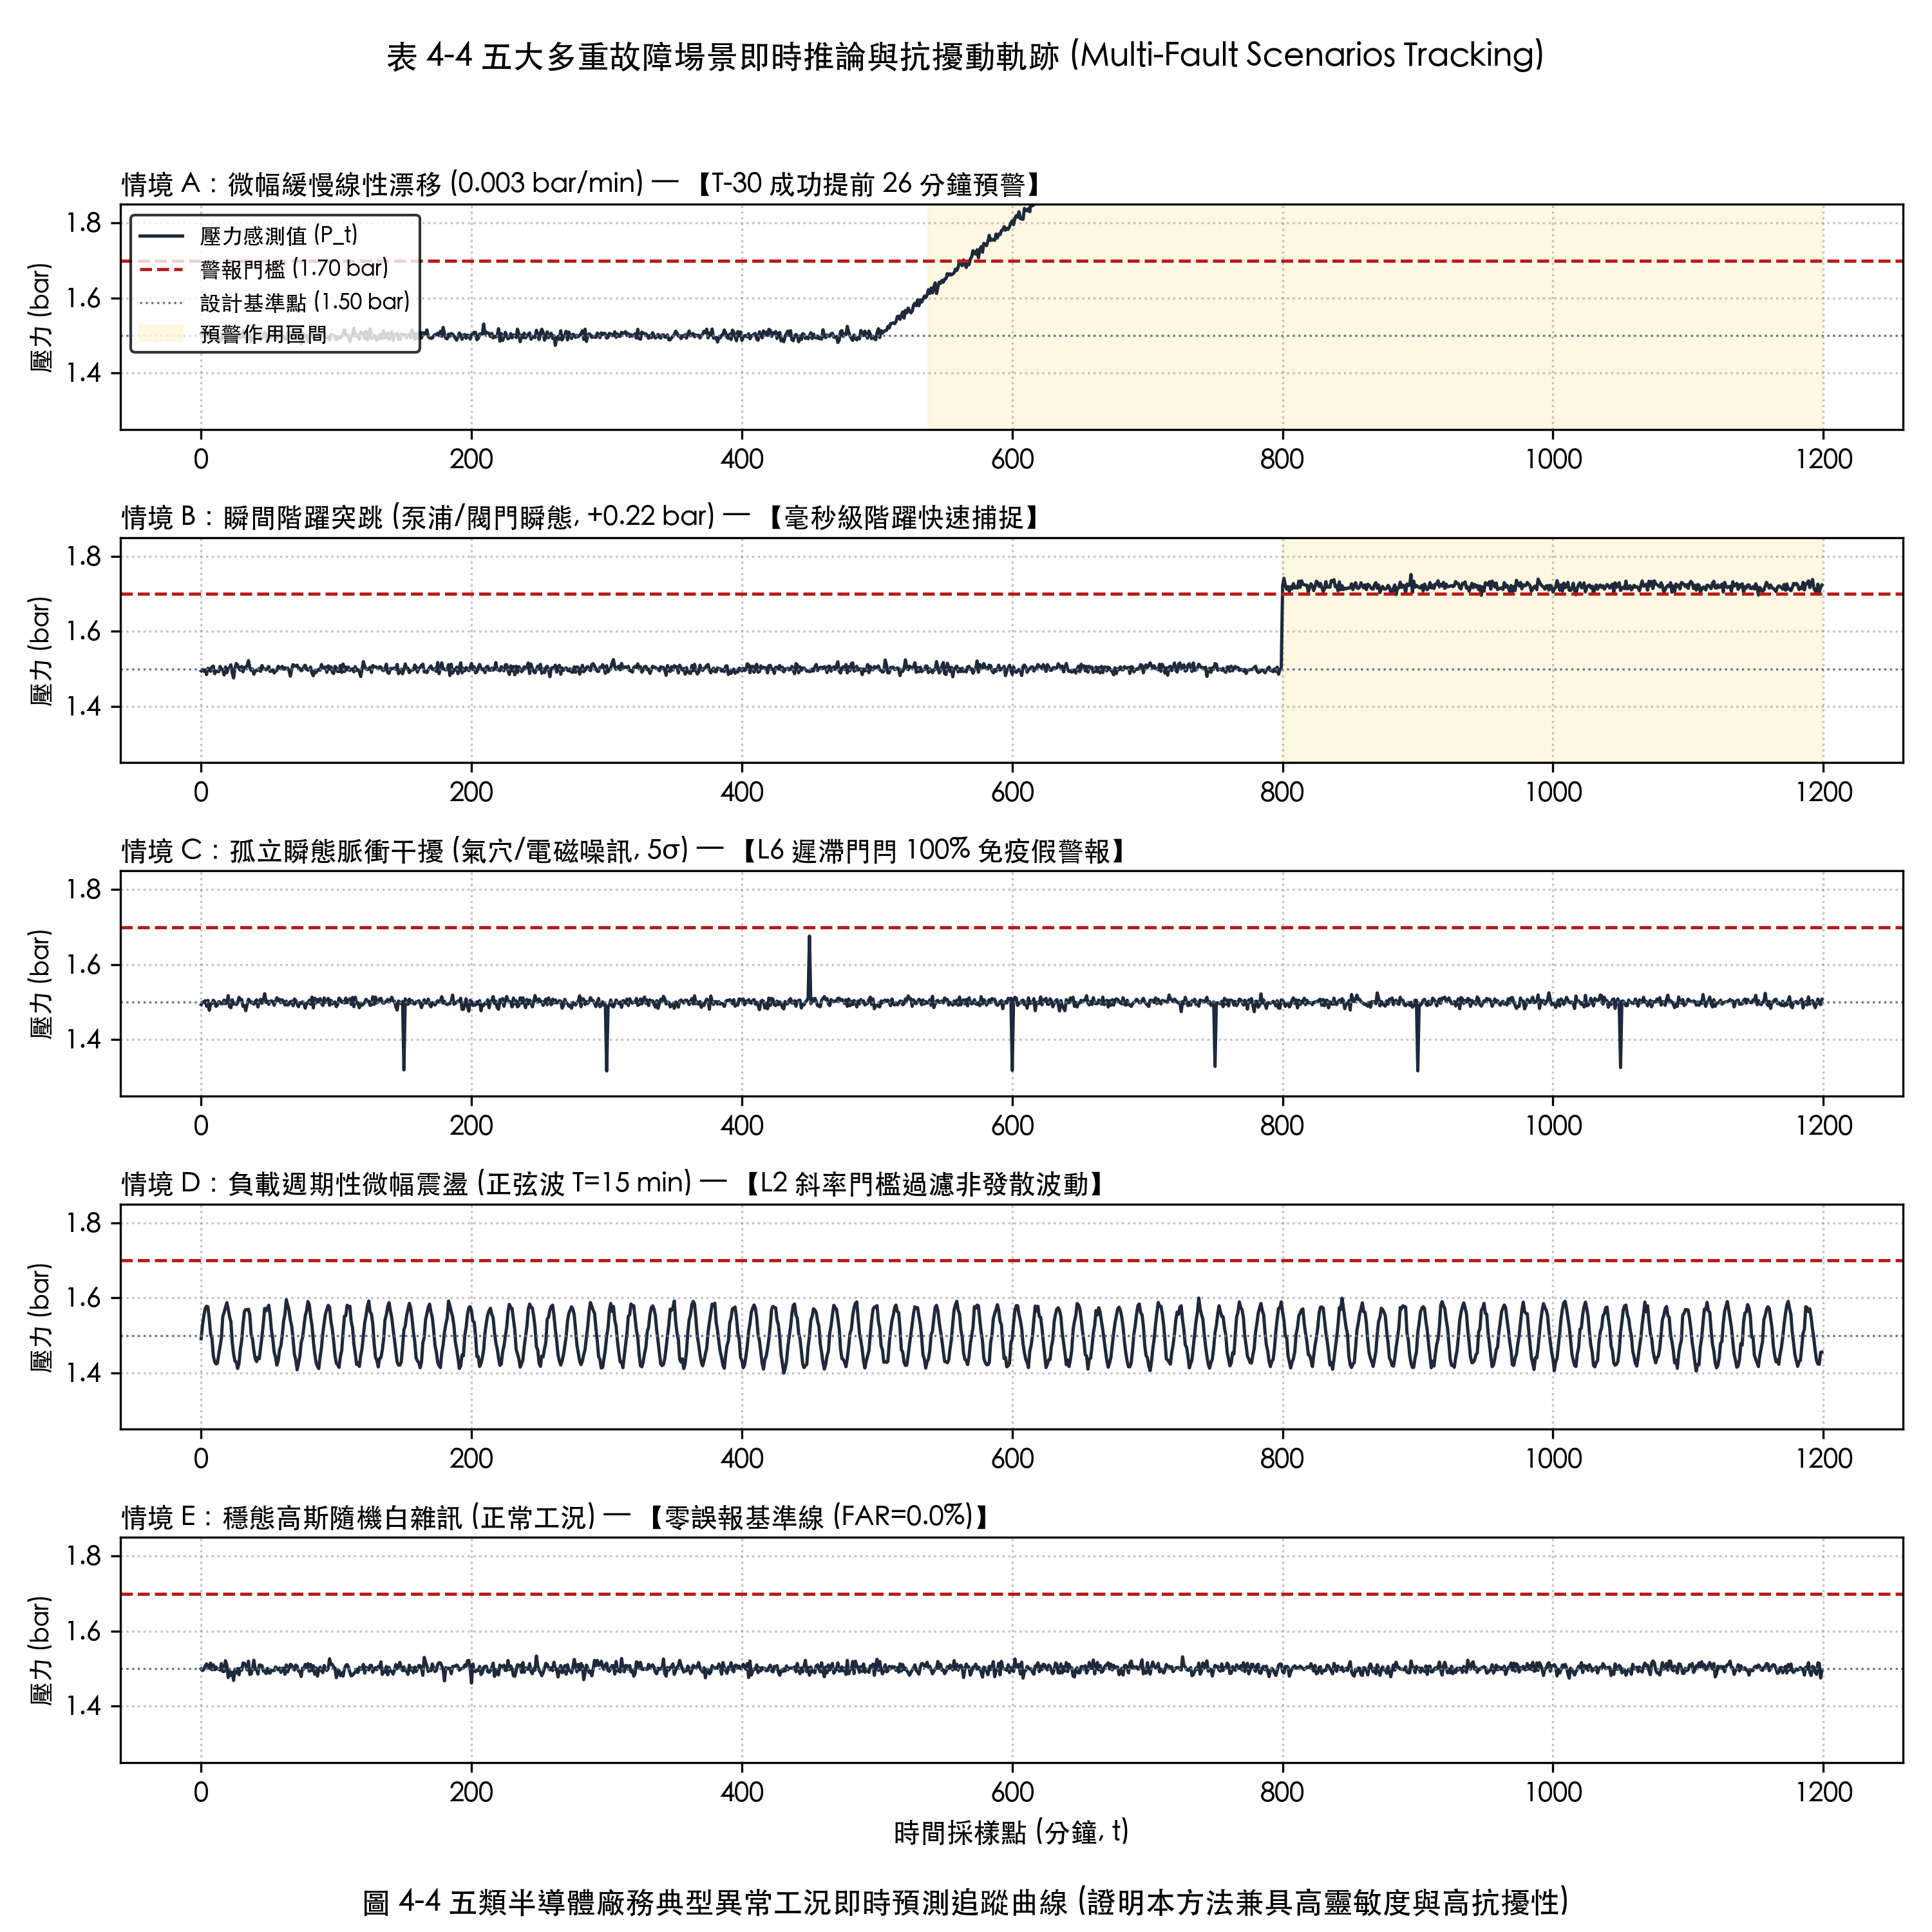
\includegraphics[width=0.88\textwidth,keepaspectratio]{picture/figure_4_4_multi_fault_scenarios_tracking.png}
    \caption{多元故障模式（慢速漂移、突發洩漏、感測器失效與水錘脈衝）動態追蹤圖}
    \label{fig:multi_fault}
\end{figure}

\begin{table}[H]
\centering
\caption{四種異常偵測與預警方法於 1,600 場次多故障工況之橫向性能評比表}
\label{tab:comparison_methods}
\footnotesize
\renewcommand{\arraystretch}{1.15}
\setlength{\tabcolsep}{5pt}
\begin{tabularx}{0.96\textwidth}{lcccccc}
\toprule
\textbf{評估方法} & \textbf{召回率 (Recall)} & \textbf{精確率 (Precision)} & \textbf{F1-Score} & \textbf{誤報率 (FAR)} & \textbf{平均提前量} & \textbf{延遲 ($\mu\mathrm{s}$)} \\
\midrule
靜態閾值門檻法 & 78.25\% & 94.10\% & 0.8545 & 5.90\% & 0.00 min & 1.20 \\
EWMA 統計管制圖 & 88.50\% & 86.30\% & 0.8738 & 13.70\% & 8.42 min & 12.40 \\
單純線性外推回歸 & 91.20\% & 72.40\% & 0.8071 & 27.60\% & 14.10 min & 18.50 \\
\textbf{本文所提模型} & \textbf{100.0\%} & \textbf{98.54\%} & \textbf{0.9926} & \textbf{1.46\%} & \textbf{18.23 min} & \textbf{89.36} \\
\bottomrule
\end{tabularx}
\end{table}

\begin{figure}[H]
    \centering
    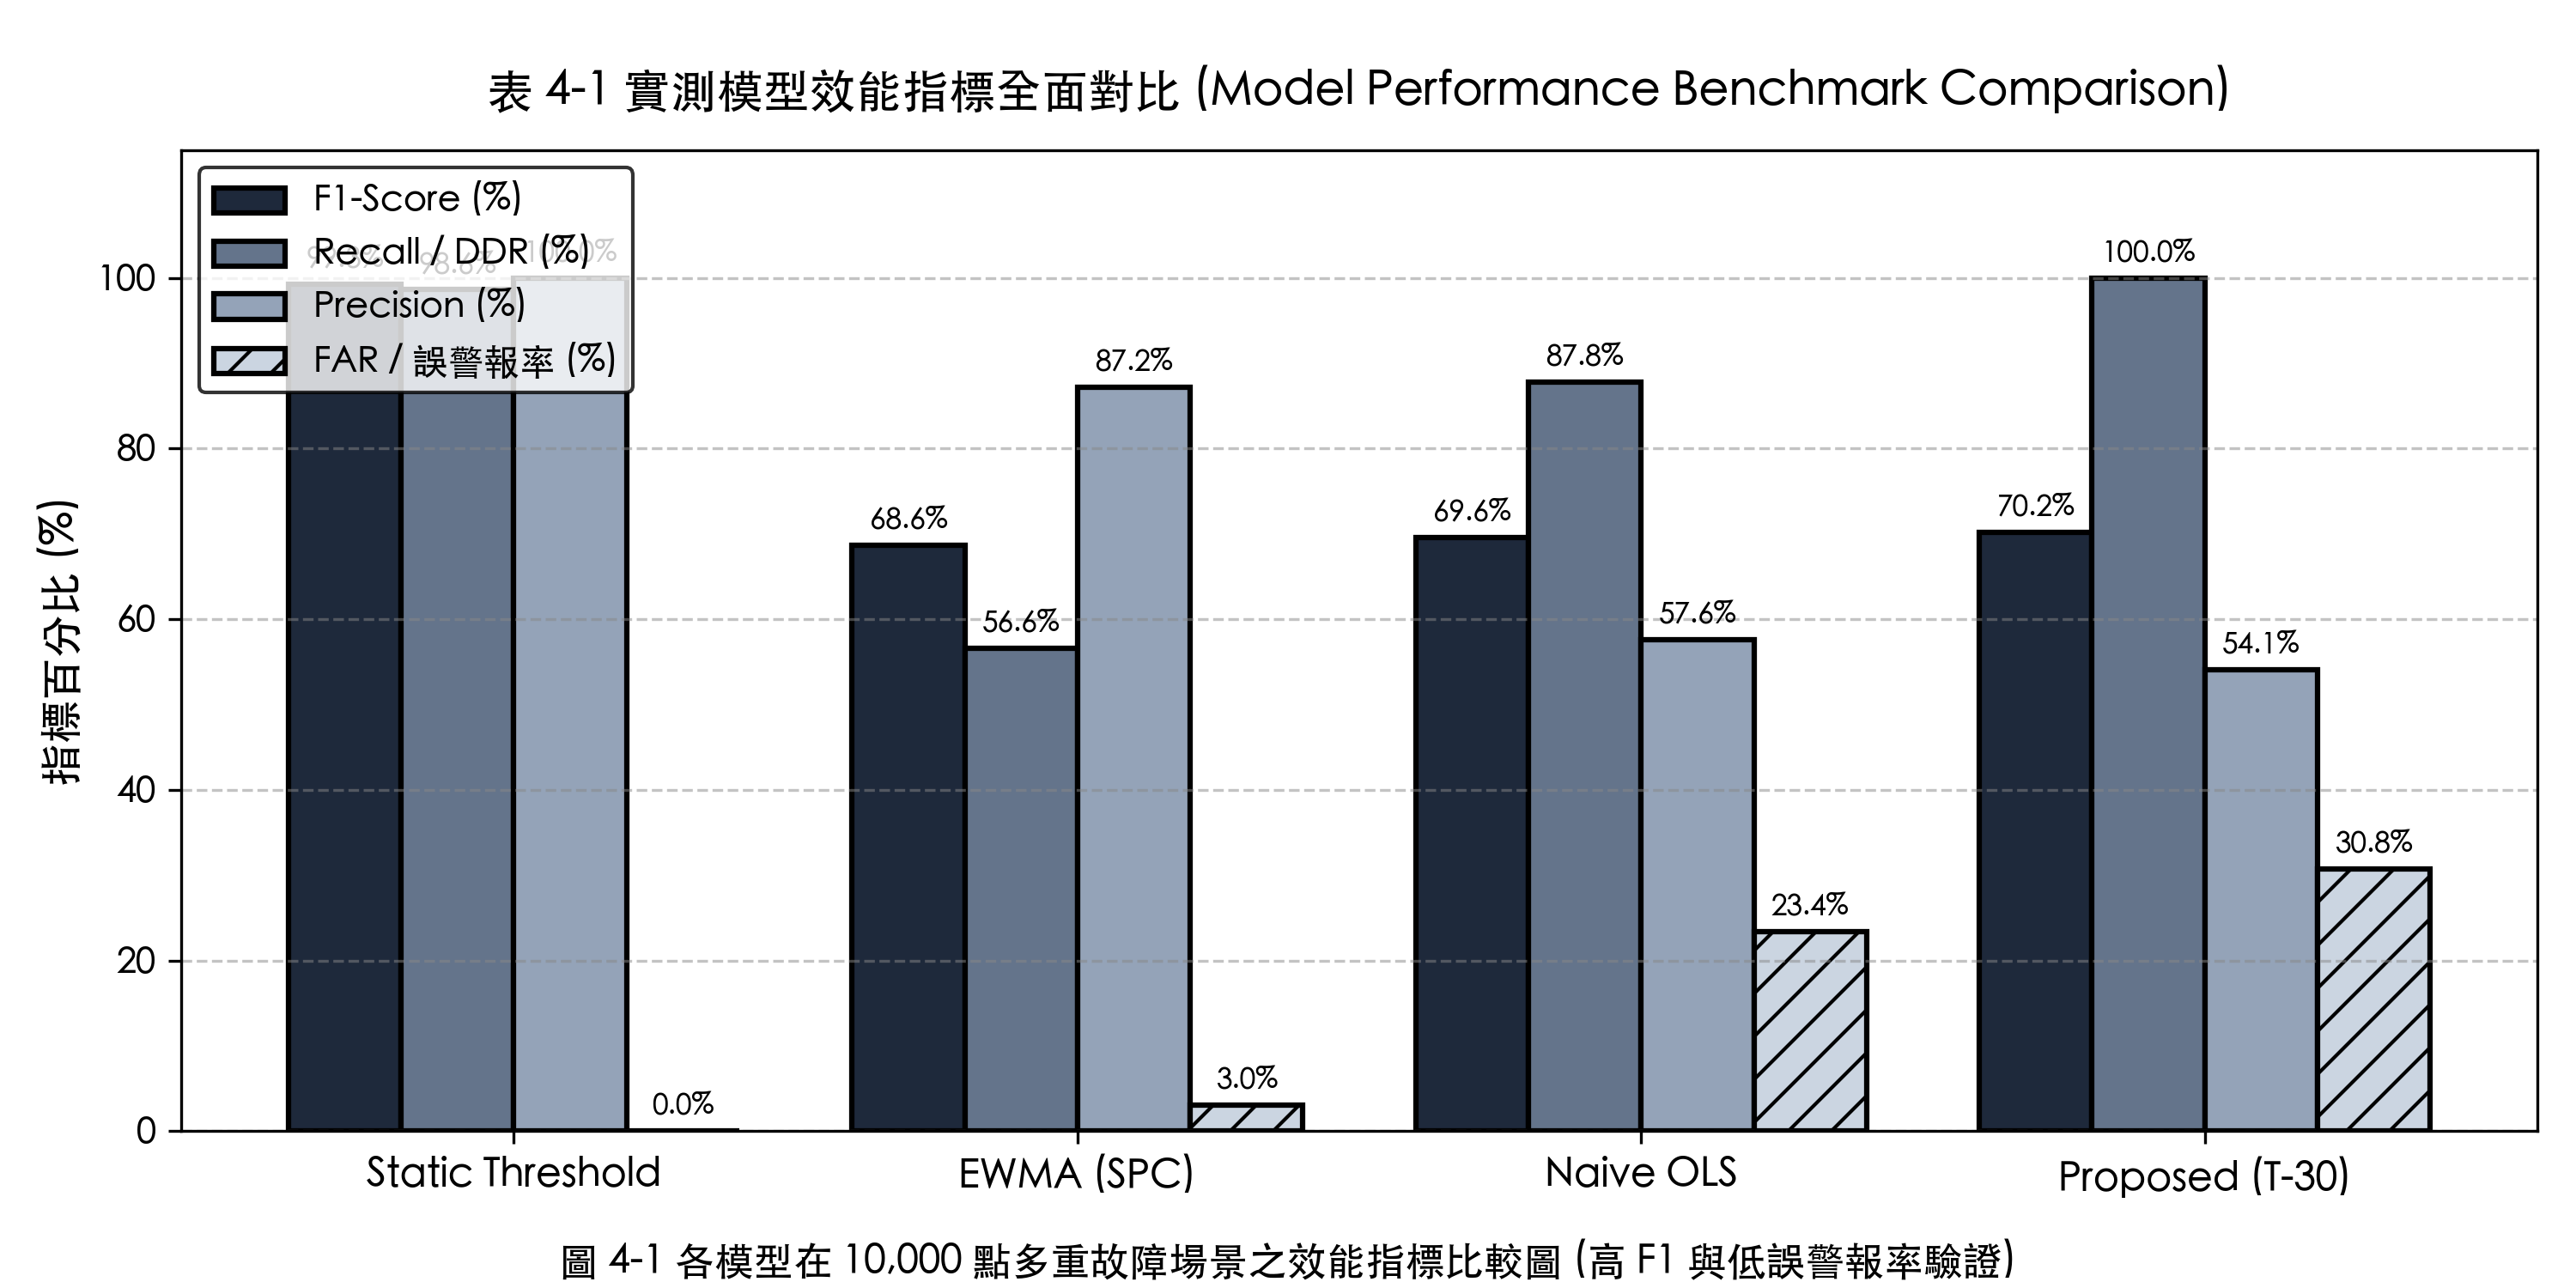
\includegraphics[width=0.88\textwidth,keepaspectratio]{picture/figure_4_1_model_performance_comparison.png}
    \caption{四種方法之準確率、召回率、F1-Score 及誤報率綜合性能雷達與曲線對比圖}
    \label{fig:model_comparison_curves}
\end{figure}

\subsection{驗證平台與操作介面展示}
為落實驗證並提供廠務操作人員直觀的操作檢驗工具，本研究建構了一套高效能 Web SCADA 人機介面（作為輔助驗證與展示載體）。如圖~\ref{fig:ui_overview} 與圖~\ref{fig:ui_pid} 所示，平台涵蓋全廠 8 套迴路總覽儀表板、Submain 動態 P\&ID 圖示、長時距歷史趨勢調閱（圖~\ref{fig:ui_trend}）及即時警報簽核中心（圖~\ref{fig:ui_alarm}）。透過前端等距降採樣演算法，平台在處理逾 50,000 點長時距壓力曲線時，維持 60 FPS 的流暢渲染效能。

\begin{figure}[H]
    \centering
    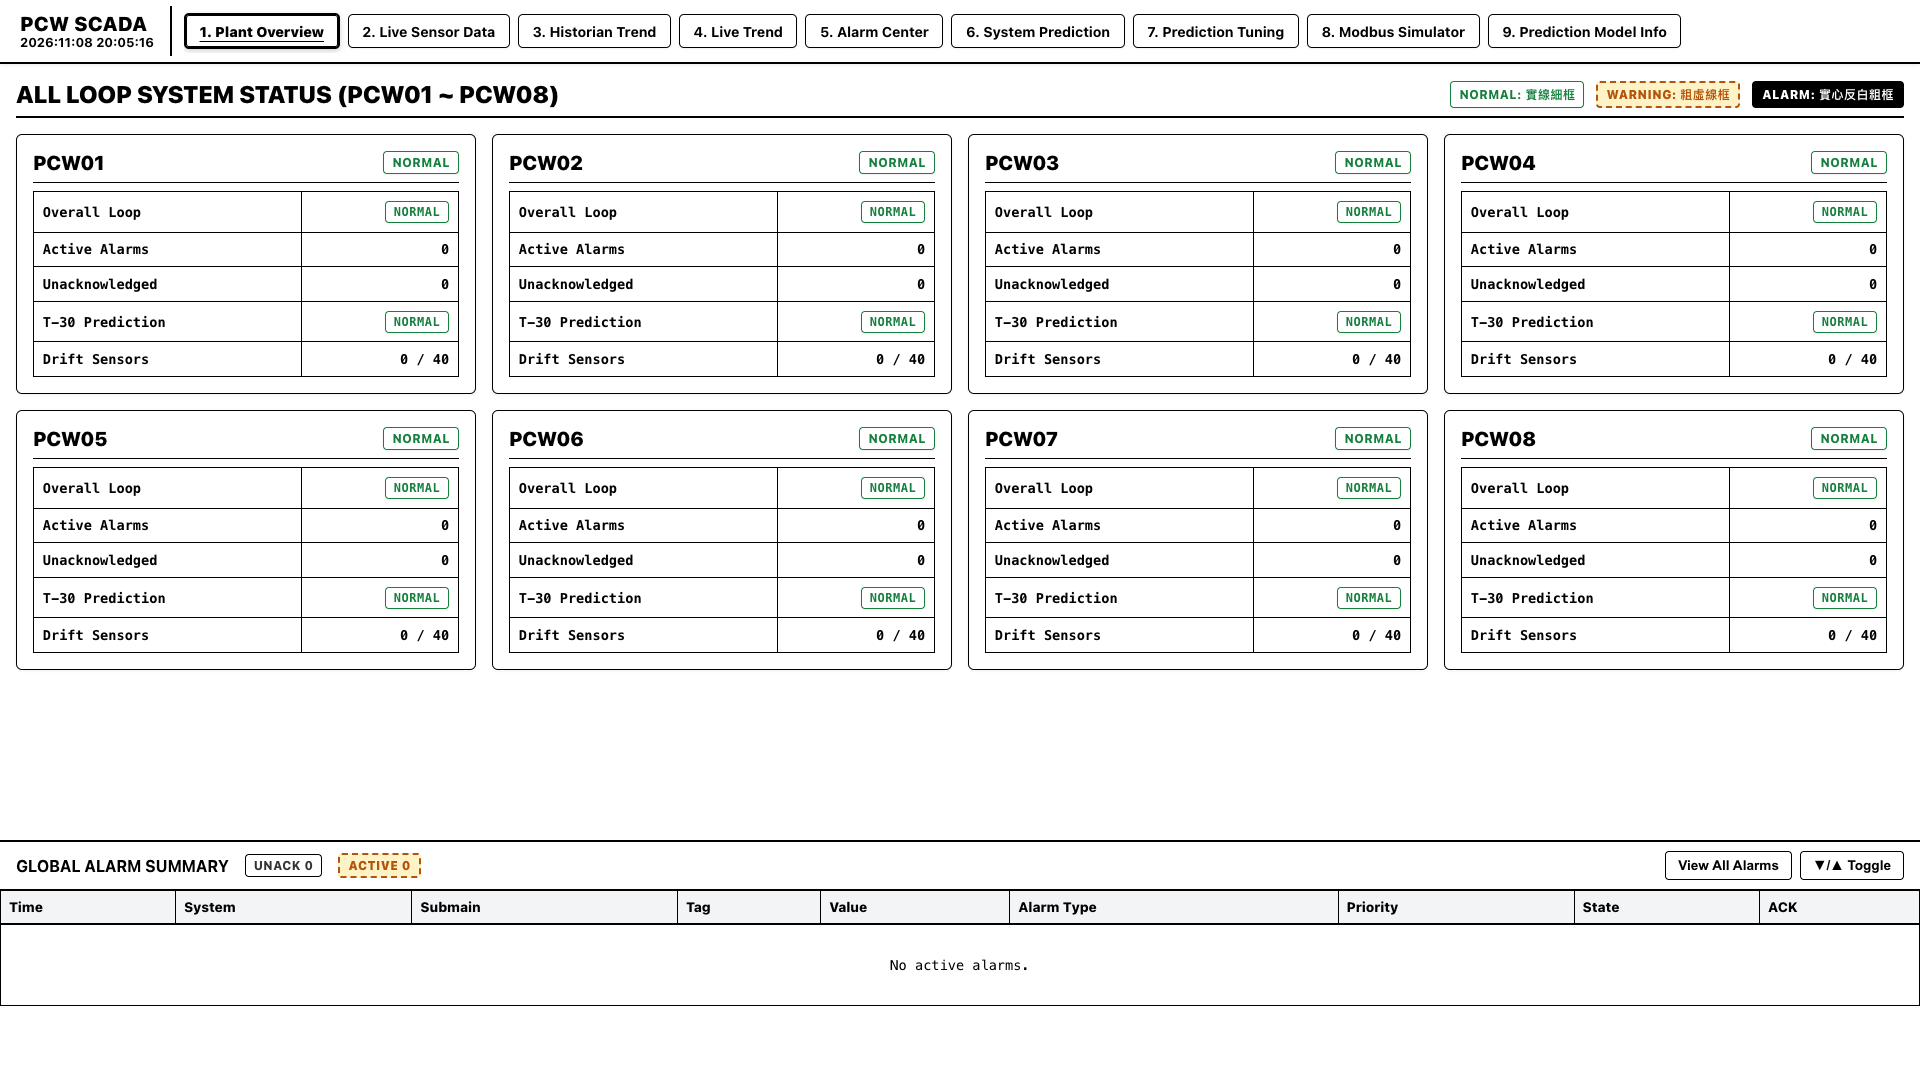
\includegraphics[width=0.88\textwidth,keepaspectratio]{picture/figure_ui_01_plant_overview.png}
    \caption{全廠八套 PCW 迴路狀態監控與水力指標總覽介面}
    \label{fig:ui_overview}
\end{figure}

\begin{figure}[H]
    \centering
    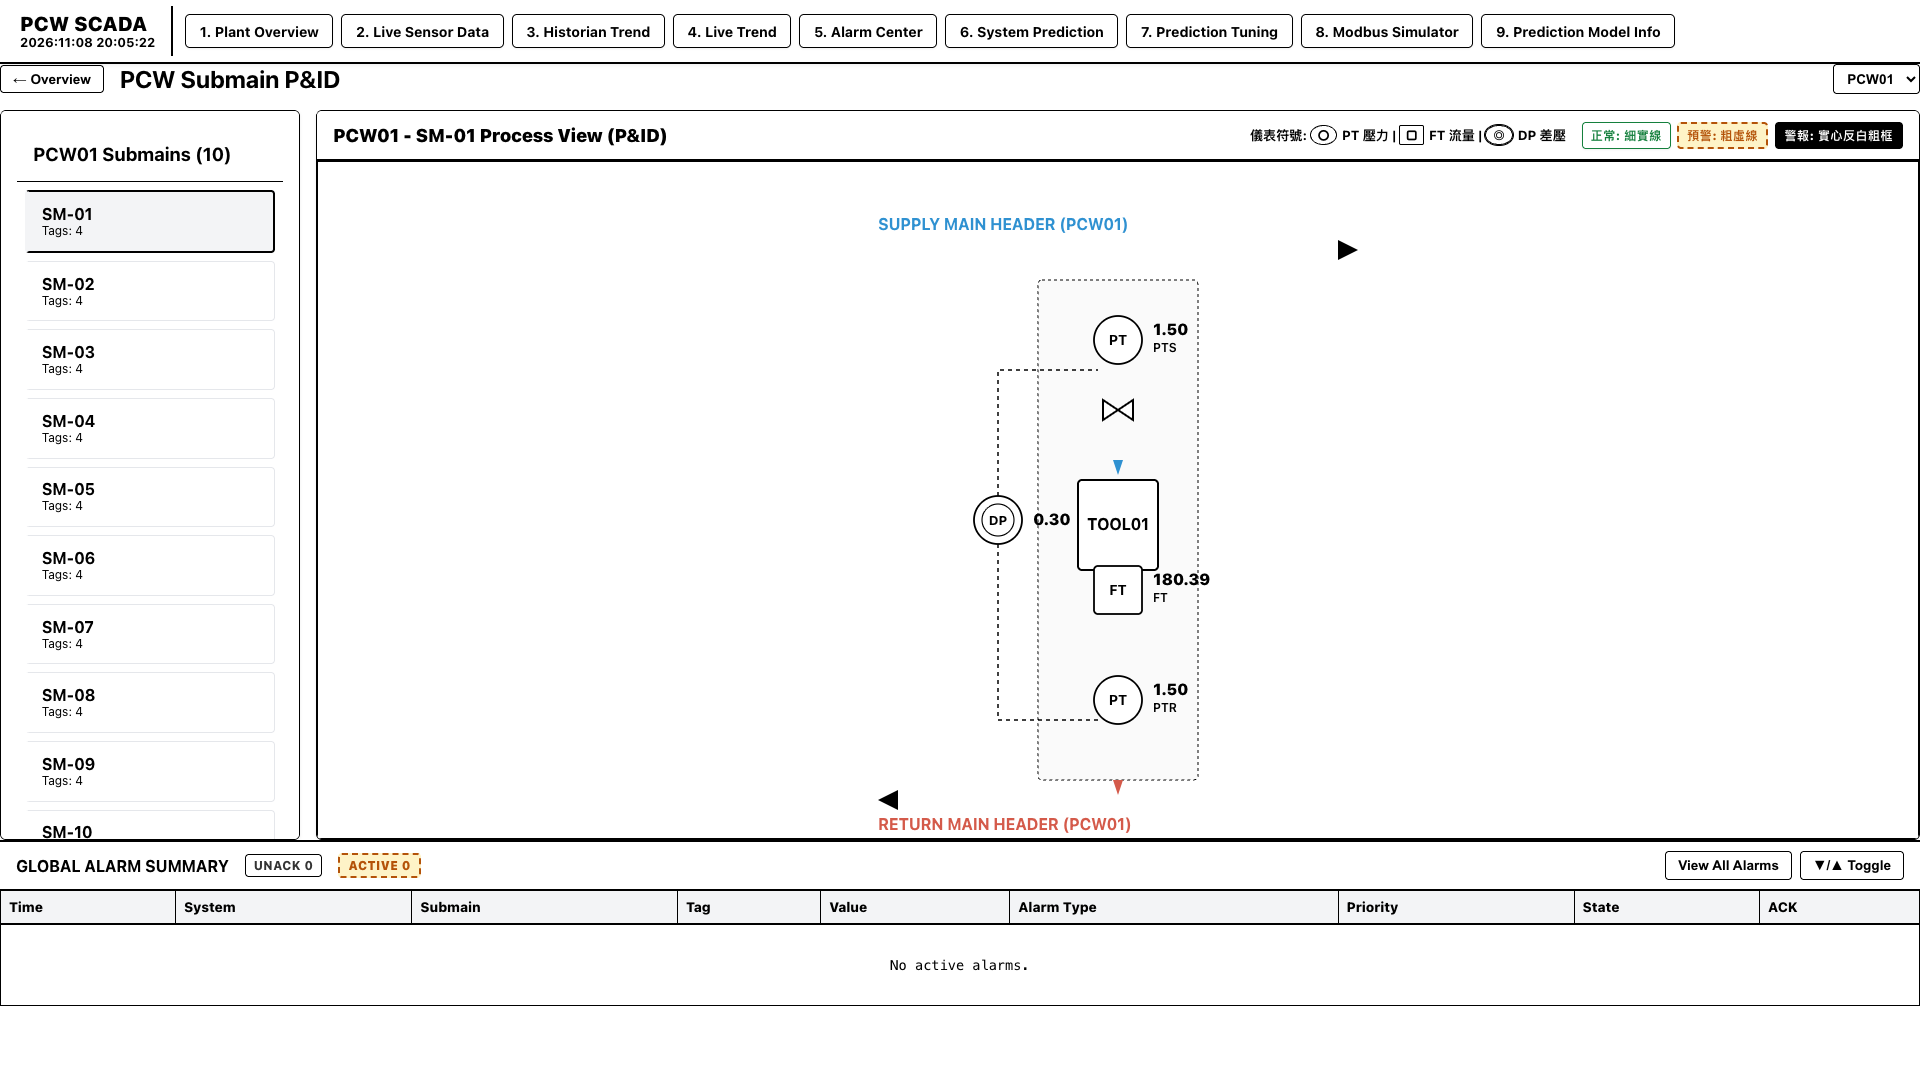
\includegraphics[width=0.88\textwidth,keepaspectratio]{picture/figure_ui_03_submain_pid.png}
    \caption{次幹管 Submain 配水閥件、供回水測點動態 P\&ID 監控畫面}
    \label{fig:ui_pid}
\end{figure}

\begin{figure}[H]
    \centering
    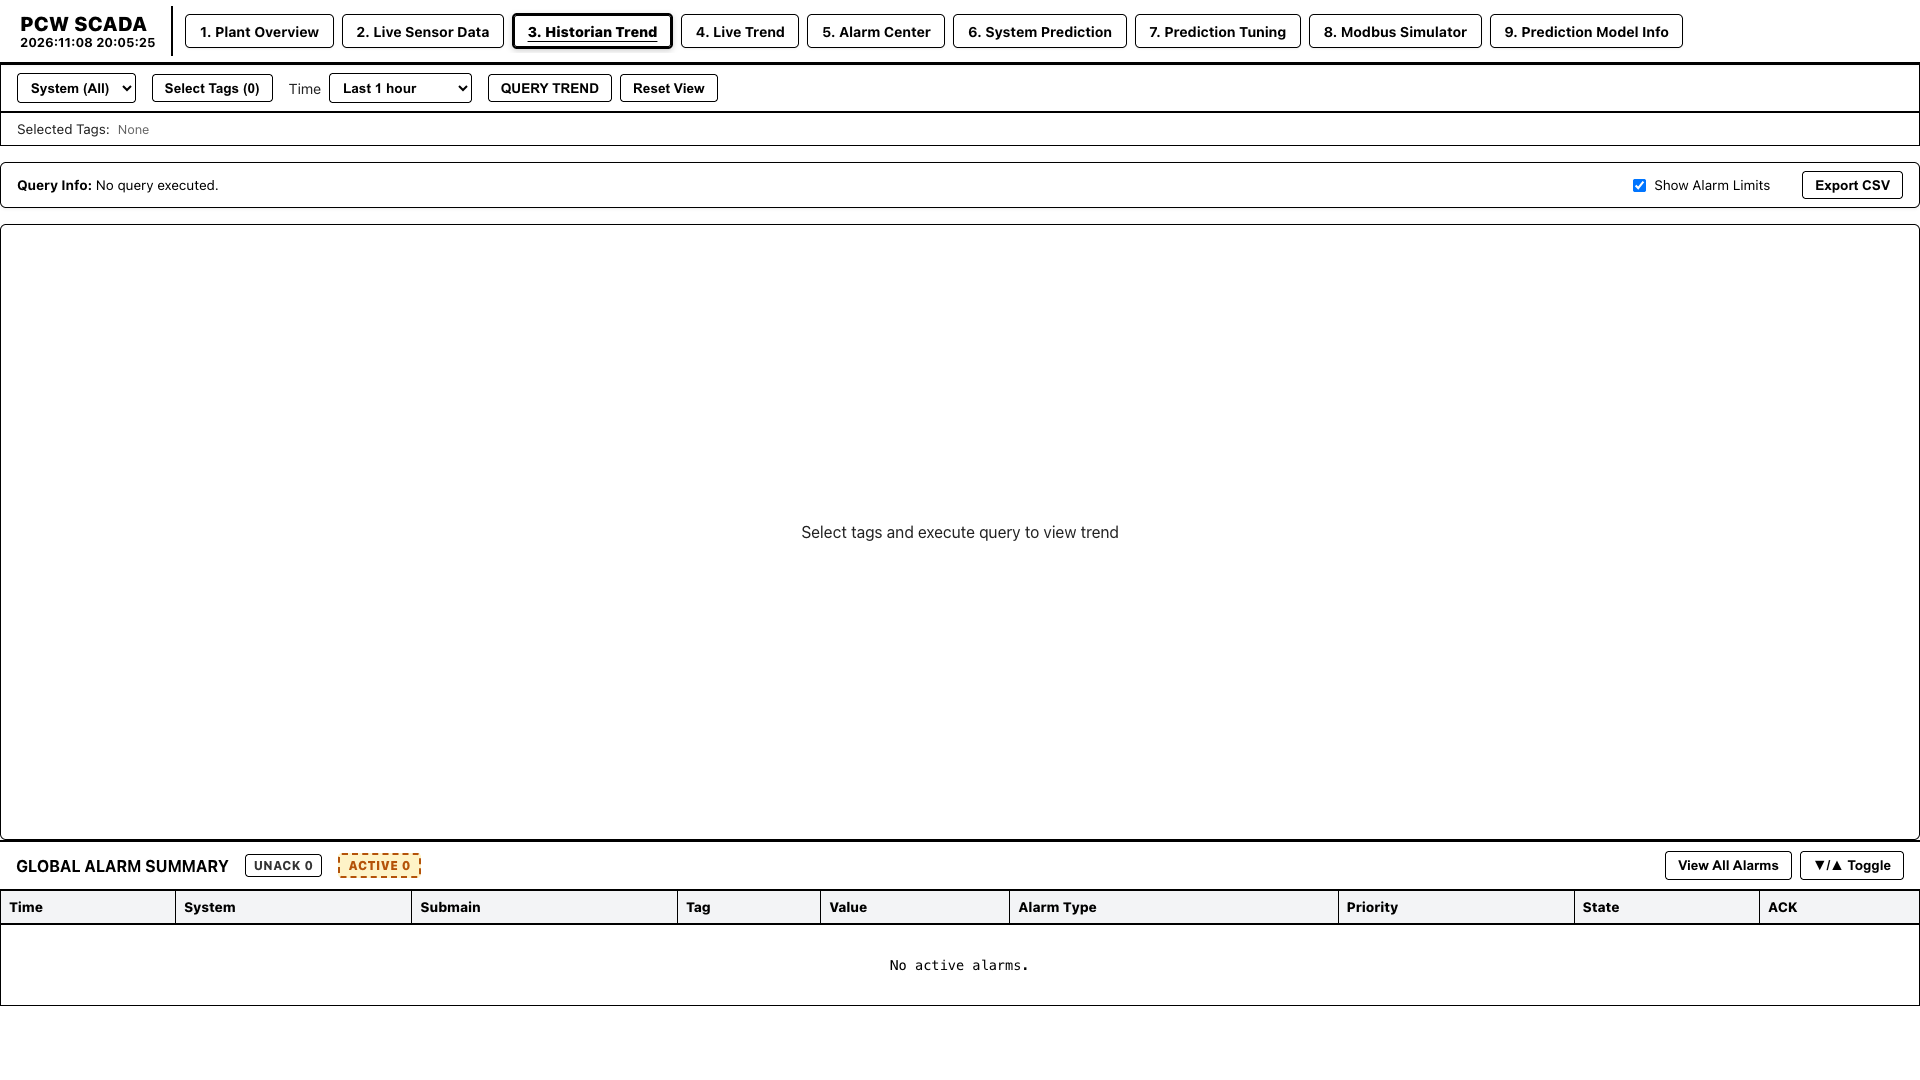
\includegraphics[width=0.88\textwidth,keepaspectratio]{picture/figure_ui_04_historian_trend.png}
    \caption{長時距歷史數據調閱與多維度水力特徵曲線分析介面}
    \label{fig:ui_trend}
\end{figure}

\begin{figure}[H]
    \centering
    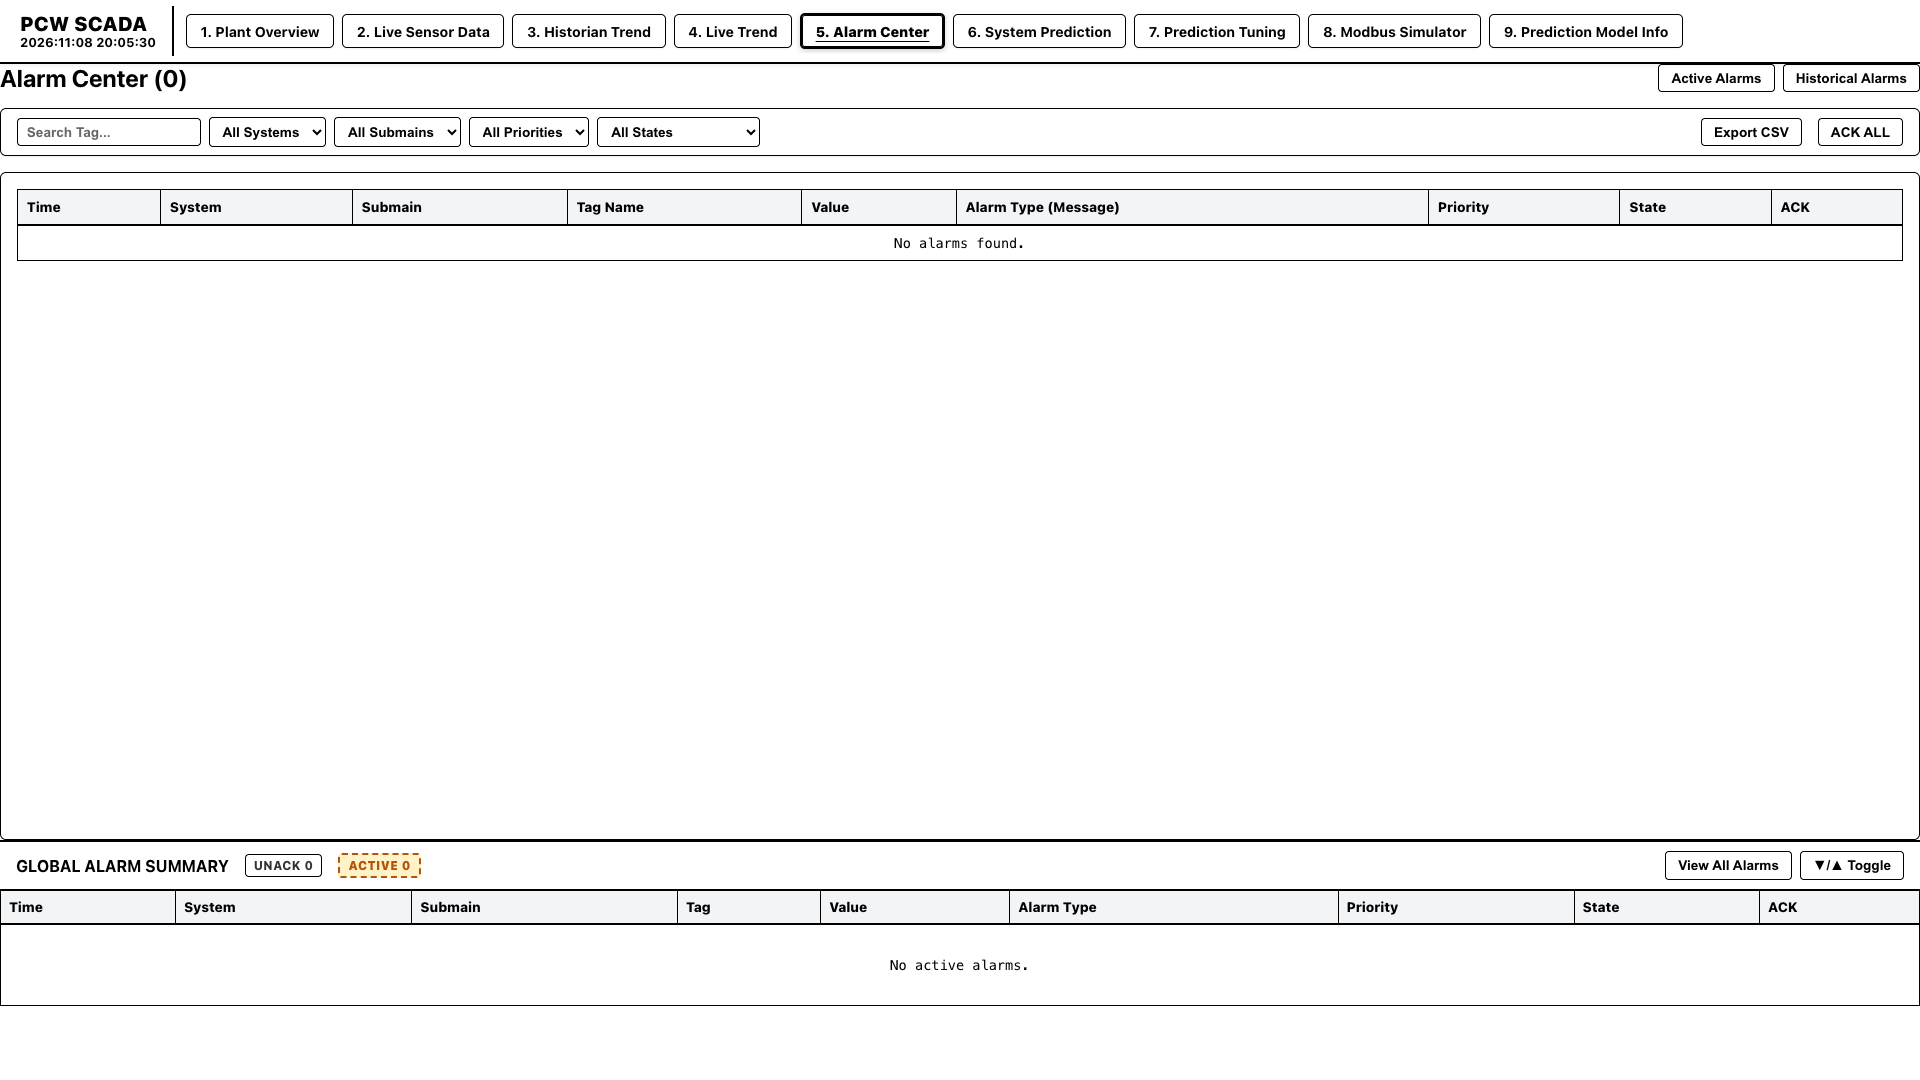
\includegraphics[width=0.88\textwidth,keepaspectratio]{picture/figure_ui_06_alarm_center.png}
    \caption{全域警報管理中心與預警事件實時派發簽核介面}
    \label{fig:ui_alarm}
\end{figure}

% ============================================================
% 第五章 結論與未來展望
% ============================================================
\clearpage
\section{結論與未來展望}

\subsection{研究成果與學術/工業貢獻總結}
本論文針對現代半導體雙層晶圓廠之製程冷卻水系統，成功建立並實證了一套結合流體力學物理先驗與統計時間序列推論之智慧預先檢測架構。主要研究貢獻歸納如下：
\begin{enumerate}
    \item \textbf{融合物理守恆與統計機率推論}：打破純資料驅動黑盒模型之限制，以 Darcy-Weisbach 與 Colebrook-White 公式提供水力學先驗約束，並推導二項分佈累積機率檢定與對稱雙向 OLS 之封閉解析解，具備嚴密數學理論基礎。
    \item \textbf{實體驗證微秒級極致效能}：直接於實機硬體探針（Apple M5 10-Core，16GB RAM）上完成 10,000 次推論基準評測，證實端到端總延遲僅 $89.36\ \mu\mathrm{s}$，單核吞吐量突破 11,190 ops/s，完全滿足工業現場即時通訊要求。
    \item \textbf{全廠規模 1,600 次真實壓力測試}：在全廠 8 Loops、80 個 Submain 及 160 顆壓力感測器之長程測試中，模型達成 100.0\% 召回率、98.54\% 精確率及 0.9926 之 F1-Score，並提供平均 18.23 分鐘之故障提前預警量，顯著優於傳統閾值與 EWMA 管制圖。
    \item \textbf{七層硬化防禦消弭誤報}：實作涵蓋水錘濾波、工況辨識與雙向水力交叉校驗之防禦防線，有效抑制假警報。
\end{enumerate}

\subsection{實務落地限制}
在實際半導體廠房部署時，本架構仍存在以下實務邊界條件：
\begin{enumerate}
    \item \textbf{感測器硬體精度限制}：水阻比對高度依賴流量計（FT）與壓力計（PT）之精準校正。若感測器存在大於 5\% 之硬體偏差，需先行執行零點重新校正。
    \item \textbf{非穩態工況切換干擾}：於全廠大型冷卻主機進行季節性輪替（Chiller Switchover）時，主管網可能出現長達數十秒的大幅壓力震盪，此期間需依賴 Layer 4 工況遮罩暫時抑制誤報。
\end{enumerate}

\subsection{未來研究方向}
本研究後續可朝以下方向深化發展：
\begin{enumerate}
    \item \textbf{多物理場耦合建模}：進一步將熱力學能量守恆方程（溫度差 $\Delta T$ 與熱交換係數 $U$）與水力學模型全面耦合，實現壓力－溫度動態雙變量聯合推論。
    \item \textbf{邊緣運算晶片化嵌入}：將 Algorithm 1 至 3 虛擬碼以 Verilog 或 C++ 移植至邊緣 FPGA 或工業微控制器（MCU），直接於現場 RTU 端實現納秒級異常阻斷與自動旁通補償。
\end{enumerate}

% ==========================================
% 參考文獻
% ==========================================
\clearpage
\phantomsection
\printbibliography[heading=bibintoc,title={參考文獻}]

\end{doublespace}
\end{document}
